\documentclass[letterpaper]{article}
\usepackage{graphicx}
\usepackage[left=3cm,top=2cm,bottom=2cm,right=3cm]{geometry}
\usepackage[title,titletoc]{appendix}
\usepackage{authblk}


\title{A Full Mesh ATCA-based General Purpose
\\Data Processing Board (Pulsar II)
\\Fermilab Technical Memo TM-2650-E}

\author[3]{Sudha Ajuha}
\author[3]{Andr\'{e} Cascadan}
\author[3]{Thiago Costa de Paiva}
\author[5]{Souvik Das}
\author[6]{Ricardo Eusebi}
\author[3]{Vitor Finotti Ferreira}
\author[4]{Kristian Hahn}
\author[1]{Zhen Hu}
\author[1]{Sergo Jindariani}
\author[5]{Jacobo Konigsberg}
\author[1]{Tiehui Ted Liu}
\author[5]{Jia Fu Low}
\author[1]{Yasuyuki Okumura}
\author[1]{Jamieson Olsen}
\author[3]{Lucas Arruda Ramalho}
\author[5]{Roberto Rossin}
\author[1]{Luciano Ristori}
\author[3]{Ailton Akira Shinoda}
\author[1]{Nhan Tran}
\author[4]{Marco Trovato}
\author[6]{Keith Ulmer}
\author[3]{M\'{a}rio Vaz}
\author[4]{Xianshan Wen}
\author[1]{Jin-Yuan Wu}
\author[1,2]{Zijun Xu}
\author[1]{Hang Yin}
\author[4,7]{Silvia Zorzetti}

\affil[1]{Fermi National Accelerator Laboratory\footnote{Operated by Fermi Research Alliance, LLC under Contract No. DE-AC02-07CH11359 with the United States Department of Energy.}, Batavia, Illinois USA}
\affil[2]{Peking University, Beijing CHINA}
\affil[3]{UNESP - S\~{a}o Paulo State University, S\~{a}o Paulo BRAZIL}
\affil[4]{Northwestern University, Evanston, Illinois USA}
\affil[5]{University of Florida, Gainesville, Florida USA}
\affil[6]{Texas A\&M University, College Station, Texas USA}
\affil[7]{CERN, Geneva SWITZERLAND}

\date{\today}


% Alter some LaTeX defaults for better treatment of figures:
% See p.105 of "TeX Unbound" for suggested values.
% See pp. 199-200 of Lamport's "LaTeX" book for details.
%   General parameters, for ALL pages:
\renewcommand{\topfraction}{0.9}	% max fraction of floats at top
\renewcommand{\bottomfraction}{0.8}	% max fraction of floats at bottom
%   Parameters for TEXT pages (not float pages):
\setcounter{topnumber}{2}
\setcounter{bottomnumber}{2}
\setcounter{totalnumber}{4}     % 2 may work better
\setcounter{dbltopnumber}{2}    % for 2-column pages
\renewcommand{\dbltopfraction}{0.9}	% fit big float above 2-col. text
\renewcommand{\textfraction}{0.07}	% allow minimal text w. figs
%   Parameters for FLOAT pages (not text pages):
\renewcommand{\floatpagefraction}{0.7}	% require fuller float pages
% N.B.: floatpagefraction MUST be less than topfraction !!
\renewcommand{\dblfloatpagefraction}{0.7}	% require fuller float pages
% remember to use [htp] or [htpb] for placement



\begin{document}

\begin{center}
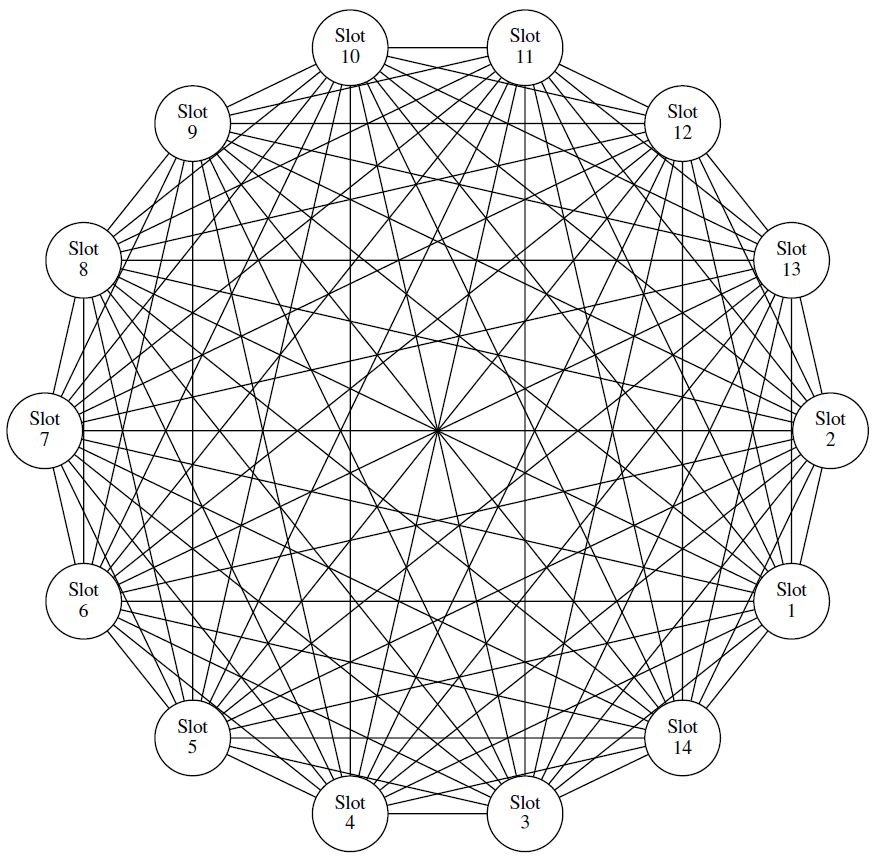
\includegraphics[width=12cm]{fullmesh.png}
\end{center}

\maketitle

% \begin{center}
% Operated by Fermi Research Alliance, LLC
% \\under Contract No. DE-AC02-07CH11359 
% \\with the United States Department of Energy.
% \end{center}

\begin{abstract}
\noindent The Pulsar II is a custom ATCA full mesh enabled FPGA-based processor board which has been designed with the goal of creating a scalable architecture abundant in flexible, non-blocking, high bandwidth interconnections. The design has been motivated by silicon-based tracking trigger needs for LHC experiments. In this technical memo we describe the Pulsar II hardware and its performance, such as the performance test results with full mesh backplanes from different vendors, how the backplane is used for the development of low-latency time-multiplexed data transfer schemes and how the inter-shelf and intra-shelf synchronization works.
\end{abstract}

\newpage
\tableofcontents

% \newpage
\listoffigures
\listoftables

% *****************************************************************************

\newpage
\section{Introduction}

Since 2012 a group of scientists and engineers at Fermilab\cite{fnal} have been involved in developing ATCA based processing boards.  These general purpose processor boards are unique in that they couple high performance FPGAs directly to the ATCA full mesh backplane; this high performance interconnect enables FPGAs in the crate to communicate directly over dedicated, non-blocking serial communication channels. Whether it's implented over a copper backplane or through optical fibers, the full mesh interconnect in effect blurs the distinction between FPGAs: full mesh architectures are uniquely suited to implement algorithms which benefit from robust data sharing across processor boundaries. Unlike bussed (PCI, VME, etc.) or star (Ethernet, PCI-e, etc.) network topologies, the full mesh interconnect is a natural fit for complex HEP applications such as trigger systems where hardware challenges are addressed through a ``divide and conquer" approach in space (detector partitioning) and time (time-muliplexing).

The focus of this technical memo is to describe in detail the Pulsar II hardware components and how they can be used to implement high performance complex systems.  We provide an example case study where the Pulsar II hardware is used to implement a low latency time-multiplexed associative-memory based level-1 track trigger demonstration system for CMS.

% *****************************************************************************

\section{Advanced Telecommunication Computing Architecture}

ATCA hardware was designed by a consortium of telecom industry leaders, and it is obvious the ATCA architecture was designed from the ground up for super reliable high availability operation.  Controller boards, power supplies, communication busses are all redundant and pratically every fan or board or module in an ATCA shelf supports hot swap insertion and removal.  In our ``bottom up" approach to hardware design we chose ATCA primarily for the unique full mesh backplane, however the robust and redundant features this architecture supports are attractive features when one considers HEP hardware is often installed in underground rooms behind interlocked doors where access is controlled.

\subsection{Specifications}

A typical 14U ATCA shelf with integrated AC-DC power supplies is shown in Figure \ref{shelf}.  Front boards measure 8U high by 280mm deep.  The board pitch is 30mm vs 20mm for VME which allows for improved airflow and taller heatsinks.  ATCA front boards are described in the PICMG 3.0 R3 specification\cite{picmg30}.  RTM boards are 8U by 72mm deep and the PICMG 3.8 specification\cite{picmg38} defines a set of power and data connectors for this board.

ATCA backplane connectors are divided into three zones.  Zone 1 consists of single large connector used for power and hardware platform management signals.  Zone 2 consists of several ADF connectors (individually shielded differential pairs, also known as ZD or ZD+) is for data transport and includes the base interface, fabric interface, and a few sets of clocks which are bussed to all slots.  (Some shelf manufacturers design separate Zone 1 and Zone 2 PCBs so that as new higher performance fabric interface designs are released they can be easily upgraded by the end user.)  Zone 3 is for user defined I/O and provides acess to the RTM board.

\begin{figure}
\centering
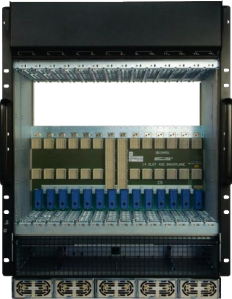
\includegraphics[width=6cm]{shelf.png}
\caption{A 14 slot ATCA shelf with integrated redundant AC-DC power supplies.}
\label{shelf}
\end{figure}

\subsection{Backplane Networks}

All ATCA backplanes have a dual star \emph{base interface} network.  The base interface is intended to be 1000BASE-T (gigabit) Ethernet, with logical slots 1 and 2 forming the hubs of the stars.  In a 14 slot shelf logical slots 1 and 2 are generally reserved for switch blades while logical slots 3-14 are reserved for processor nodes.  The base interface is intended to be used for slow control operations such as downloading FPGAs, reading and writing to status/control registers and buffers, etc.

The higher speed backplane traffic takes place on the \emph{fabric interface} which is generally offered in full mesh\ref{fullmesh} and dual star varities.  Unlike the base interface, the fabric interface does not specify a data protocol.  Each fabric interface channel is simply 4 bidirectional 100 ohm differential pairs and signal levels, data speeds, encoding, etc. are left up to the user.  Subsequent backplane generations have pushed the fabric interface performance from 10G (2.5Gbps x 4) to 40G (10Gbps x 4) to 100G (25Gpbs x 4).  In section \ref{link_perf} we chronicle our testing of the latest high performance full mesh ATCA backplanes.

\begin{figure}
\centering
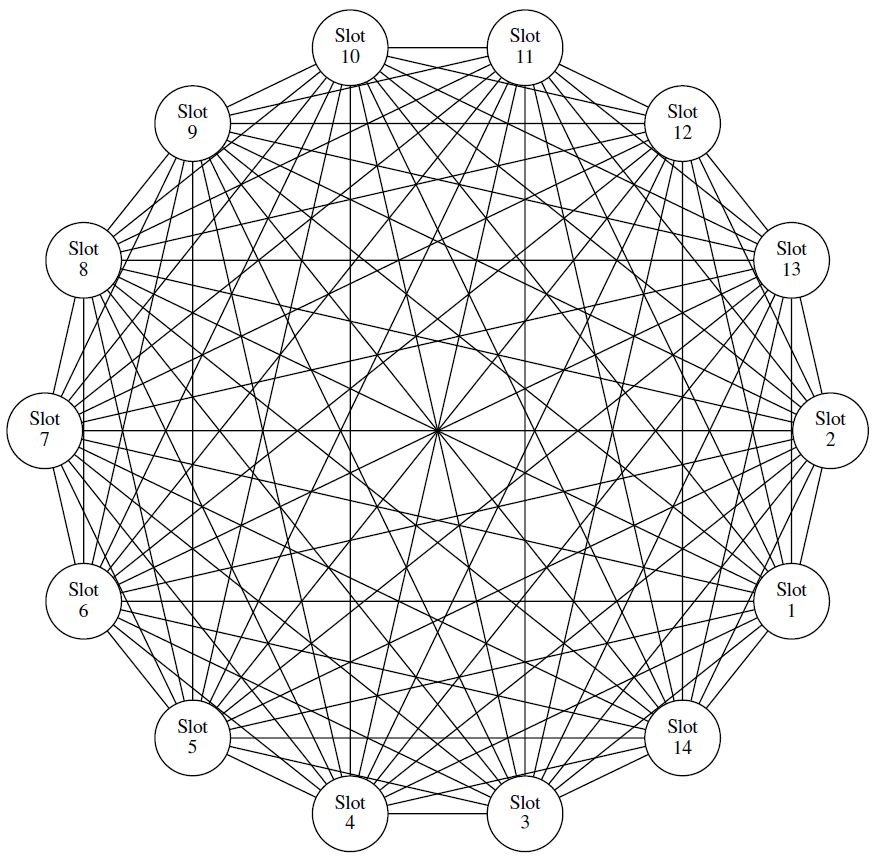
\includegraphics[width=8cm]{fullmesh.png}
\caption{Full mesh backplane connections in a 14 slot shelf.  Each line represents 4 bidirectional lanes.}
\label{fullmesh}
\end{figure}

\subsection{Hardware Platform Management}

Instrumentation and telemetry are pervasive in the ATCA shelf.  Dual redundant single board computers called shelf managers (ShMM) communicate with intelligent shelf components over redundant I2C busses and use the Intelligent Platform Management Interface protocol.  This means that most ATCA components, including fans, boards, power entry modules, and even the backplane itself are required to have at a minimum an I2C ROM which contains manufacturer data, serial numbers, etc. that the ShMM can read.  More complex modules such as boards require a microcontroller to handle more complex IPMI command sequences such as negotiating hot swap sequences and reading sensor data.

Shelf manager boards run a version of Linux and therefor it's possible to SSH into the active ShMM to manually control the fan speed, or query the health of any shelf component.  Everything is logged and recorded, so it's very useful when one needs to go back and identify a bad sensor reading and what action was taken by the ShMM.  Other useful manual ShMM operations are generating a hard reset to a particular board or cycling the power to a board.  The ShMM software is written by Pigeon Point and modified by the shelf manufacturer for their specific products (for example, shelves differ in the number and types of fans).  The PICMG specification does not define the ShMM mechanical dimensions, connectors, and mounting location, and thus most ShMM boards are unique and tied to a particular shelf design.

\subsection{Power and Cooling}

Power distribution in an ATCA shelf is similar to other telecommunications equipment which historically uses a -48VDC bus.  Dual redundant power feeds are present on the ATCA backplane and OR-ing diodes are required to provide automatic switch-over from one feed to another in the event of a sudden power loss.  Multiple large value capacitors should be located where the power enters the board.  These capacitors should be sized so that the board can ride out a 5ms power loss without any impact on board performance.  Dual power input feed or-ing diodes, filters and capacitor switchover circuitry are combined on a small Power Interface Module (PIM).

Most ATCA shelf designs have the option of including slots for N+1 redundant AC-DC power supplies on the bottom of the shelf.  These power supplies usually add 1U of vertical height of the shelf and have the AC plugs in the back.

A typical ATCA shelf pulls air in from the front, up through the boards, and exhausts out the top rear.  Fans are usually located in top of the chassis, therefore all empty slots in the front and rear of the chassis must be filled with blank panels to prevent air leakage.  Baseline thermal performance is 300W per slot, with newer high power shelves claiming over 500W per slot.  The ShMM queries all intelligent FRUs in the shelf and adjusts the fan speed and attempts to keep all temperature sensors below threshold.  Fans are removable and hot swappable.  You don't want to be in the room without hearing protection when the fans are at maximum speed.

% *****************************************************************************

\section{Pulsar IIb Front Board}

The Pulsar2b Front Board is a custom ATCA full mesh enabled FPGA-based processor board which has been designed with the goal of creating a scalable architecture abundant in flexible, non-blocking, high bandwidth interconnections.  Initially motivated by silicon-based tracking trigger needs for LHC experiments, the Pulsar2b is uniquely positioned as a flexible R\&D platform ideally suited to situations where multiple processing engines are tightly coupled.  The full mesh backplane interconnections provide an option whereby the firmware designers can effectively blur the distinction between FPGAs, and the Pulsar2b opens up options for data sharing in both space and time.  The Pulsar II hardware components are shown in Figure \ref{pulsar2} and the Pulsar2b front board block diagram is shown in Figure \ref{pulsar2b_block}.

\begin{figure}
\centering
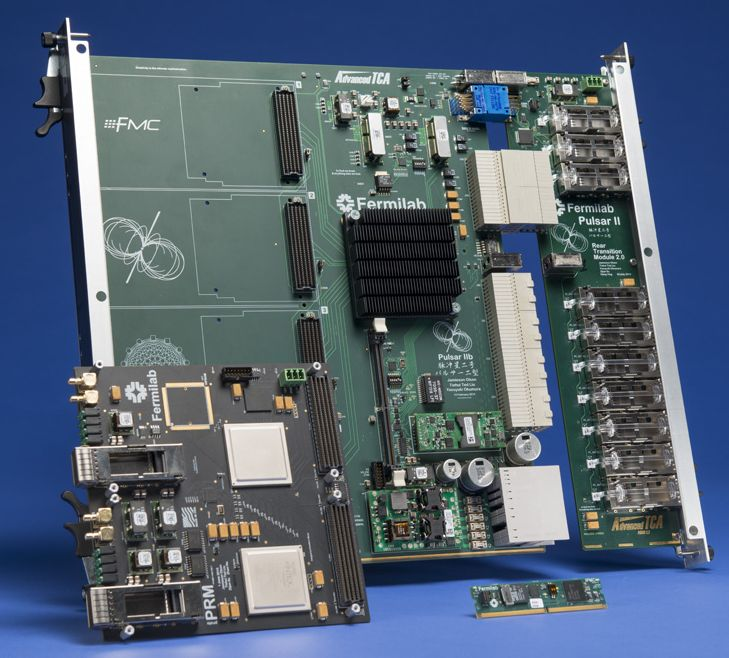
\includegraphics[width=12cm]{pulsar2.jpg}
\caption{The Pulsar IIb front board, RTM, IPMC and PRM mezzanine.}
\label{pulsar2}
\end{figure}

\begin{figure}
\centering
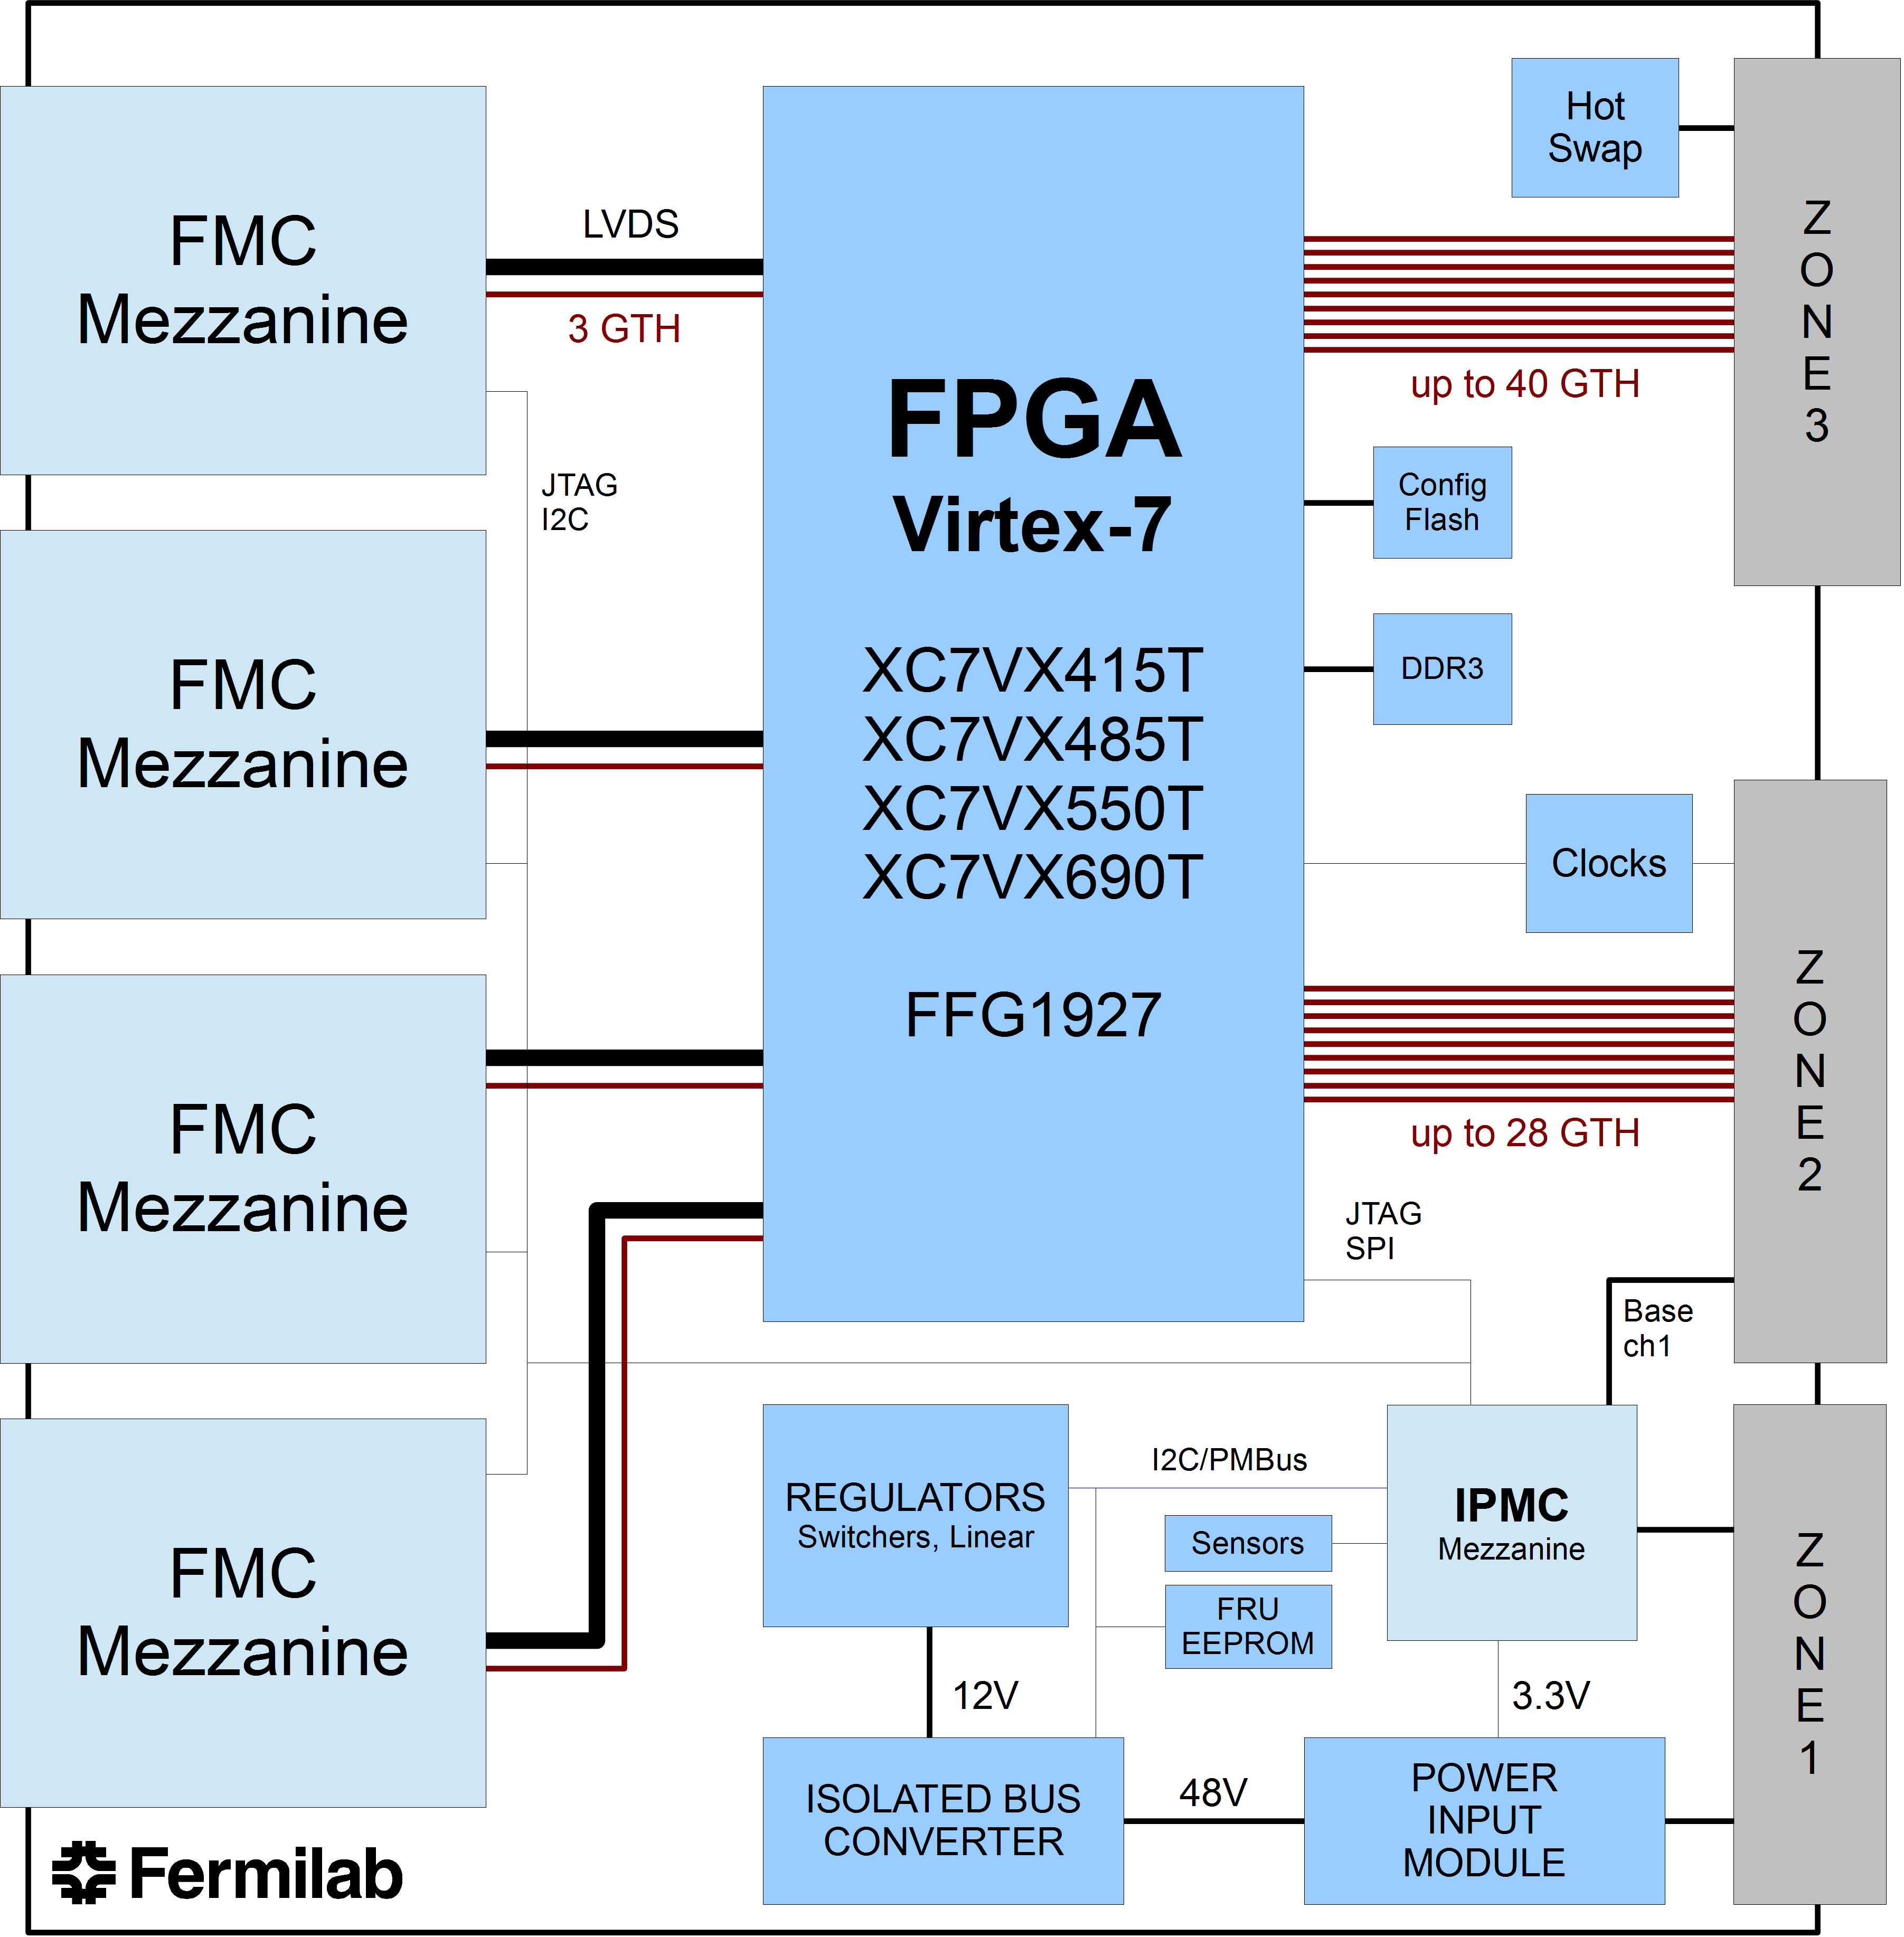
\includegraphics[width=10cm]{pulsar2b_block.png}
\caption{The Pulsar IIb front board block diagram.}
\label{pulsar2b_block}
\end{figure}

\subsection{FPGA}

A single large FPGA forms the heart of the Pulsar2b board.  The board has been designed to support a mid-size Xilinx Virtex-7 class FPGA device in the FF1927 footprint \cite{xilinx}.  Compatible FPGAs include \texttt{XC7VX415T}, \texttt{XC7VX485T}, \texttt{XC7VX550T}, and \texttt{XC7VX960T}.  To date all Pulsar2b boards have been assembled with the largest supported device \texttt{XC7VX690T-2FFG1927C} (-2 is the mid speed grade).  The \texttt{XC7VX960T} device features 693k logic cells, 3600 DSP slices, 52Mbits of dual port BlockRAM, and 80 GTH transceivers which support line rates up to 11.3Gbps.  

Worst case power dissipation in the FPGA is on the order of 60W with approximately 40W going for the transceivers and 20W for the regular I/O and core logic.  In general we have found that the actual power usage agrees well with the Xilinx power estimator spreadsheet.  A passive 70mm square heat sink is attached to the FPGA and Pulsar2b board.  A sensor on the Pulsar2b enables the IPMC to monitor the FPGA die temperature (the FPGA does not need be initialized).  This temperature reading is passed on from the IPMC to the shelf manager, which controls the shelf fan speed to insure that all temperature readings on the Pulsar2b board fall within nominal ranges.

\subsection{RTM Interface}

Ten quad small form factor pluggable transceivers (QSFP+) are located on the RTM.  When fully loaded with QSFP+ modules the RTM will support an aggregate bandwidth of 400 Gbps input and output.  AC coupling capacitors (which are required when interfacing to the FPGA MGT TX/RX pins) are located in the QSFP+ transceiver and thus are not placed on the Pulsar IIb which leads to a cleaner layout.  Since the Pulsar2b FPGA is connected directly to the QSFP+ transceivers the full diagnostic capabilities of the MGTs may be used to evaluate the quality of the RTM links at speeds up to 10Gbps.  RTM design details are provided in section \ref{rtm_section} and link performance results are summarized in section \ref{link_perf_rtm}.

\subsection{Fabric Interface}

On the Pulsar2b board up to 28 MGT transceivers are routed directly to the Zone 2 full mesh fabric interface.  Per the PICMG ATCA specification a backplane channel consists of 4 bidirectional serial ports (lanes).  On the Pulsar2b board these backplane channels are partially loaded: on channel 1 all four ports are used while channels 2 through 13 have only two ports (0,1) used.  

Xilinx strongly recommends that all MGT TX and RX data pairs should be AC coupled for proper operation.  On ATCA blades the recommendation is to incorporate these AC coupling capacitors on the RX signal pairs coming onto the board from the Zone 2 connectors.  The addition of discrete surface mounted capacitors into the high speed data path requires careful PCB layout to minimize attenuation, crosstalk and reflections from impedance discontinuities.

The direct connection to the full-mesh fabric enables the full diagnostic capabilities of the MGT transceivers to evaluate the quality of the full-mesh links at speeds up to 10 Gbps.  Communication between Pulsar2b boards has been sucessfully tested across the entire width of the ATCA backlane with line rates up to 10Gbps.  For a summary of the backplane link testing refer to Sections \ref{link_perf_40g} and \ref{link_perf_100g}.

\subsection{Mezzanine Cards}

The Pulsar IIb supports up to four FPGA Mezzanine Cards (FMC) with the high pin count (HPC) connectors.  Mezzanine cards may contain FPGAs, ASICs, optical transceivers, or any other custom hardware.  Each FMC mezzanine card connector is wired directly to the main FPGA on the Pulsar2b and supports 36 user-defined LVDS pairs and 3 10Gbps serial bidirectional lanes.  Per the VITA 57.1 specification an FMC mezzanine card is limited to approximately 35W.  On the Pulsar2b we have added a few extra 12VDC pins on a small connector next to each FMC connector to increase the power available to the mezzanines.  Mezzanine cards are connected to the Pulsar2b JTAG bus and support local and remote programming over the network through the IPMC.  A general purpose I2C bus connects each mezzanine card to the main FPGA on the Pulsar2b.

\subsection{FPGA Configuration}

Upon powerup the Pulsar2b FPGA will attempt to load a bitstream from the on-board SPI flash memory device.  At any time the Pulsar2b FPGA may be reconfigured via the JTAG bus.  The JTAG bus connects the Pulsar2b FPGA and the four FMC mezzanines in a daisy chain.  If a programming cable is connected to the JTAG header on the Pulsar2b the cable will act as the master of the JTAG bus.  Otherwise, the IPMC module acts as the JTAG bus master and allows for remote programming over the network using the Xilinx Virtual Cable (XVC) protocol.

The JTAG bus is a daisy chain.  If a mezzanine card is not installed or if the installed mezzanine does not support JTAG the user must manually set the JTAG jumper for that mezzanine connector to the BYPASS position.  JTAG signals to the mezzanine cards are 3.3V LVTTL levels.

\subsection{Backplane Synchronization Interface}
\label{section_bp_sync}

The ATCA backplane synchronization interface consists of six LVDS pairs bussed to all slots across the backplane.  The first four clock pairs (CLK1A, CLK1B, CLK2A, and CLK2B) are reserved for weird low frequency clocks that only telecom idustries care about.  The remaining two clock pairs CLK3A and CLK3B are user defined.  A pair of M-LVDS transceivers are used to interface the CLK3A and CLK3B backplane clocks to the Pulsar2b FPGA as shown in Figure \ref{sync}.

\begin{figure}
\centering
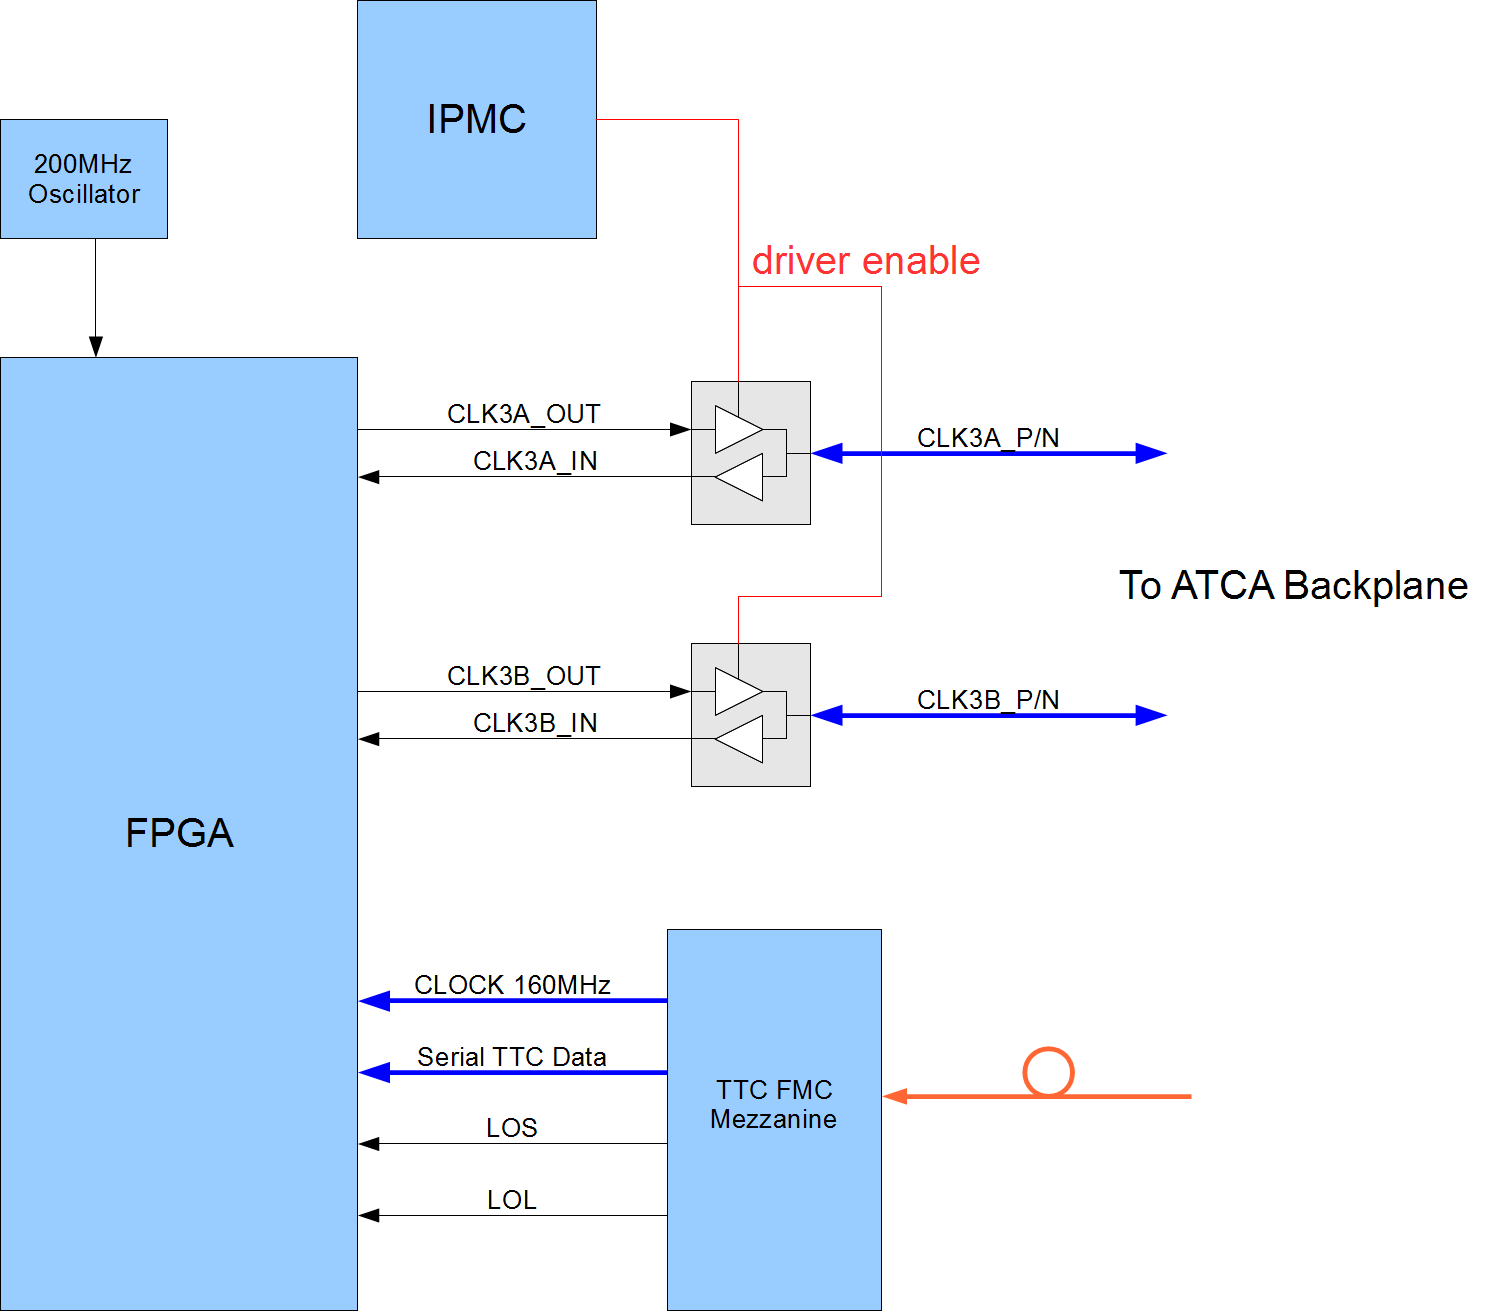
\includegraphics[width=10cm]{sync.png}
\caption{The Pulsar IIb synchronization interface.}
\label{sync}
\end{figure}

The M-LVDS receivers are always enabled and pass the CLK3A and CLK3B signals to the FPGA.  The IPMC mezzanine controls the M-LVDS drivers and it is expected that ONE and ONLY ONE Pulsar2b board in the shelf will be designated as the clock master.  Since the drivers are M-LVDS no physical damage will occur if two or more Pulsar2b boards enable the clock drivers, however.

Tests performed at Fermilab and Northwestern University show good performance on the clock signals at clock rates up to 100MHz.  Typically we run these clocks slower, using the accelerator bunch crossing clock (typically ~40MHz) as the common source to synchronize not only the Pulsar2b boards in the shelf, but Pulsar2b boards in multiple shelves as well.

The backplane clocks are not designed to be precise low-skew low-jitter clock resources.  Their main purpose is to keep all Pulsar2b boards in the system aligned to better than a few nanoseconds and provide a common frequency locked reference for all boards to use.  Internally the Pulsar2b FPGA uses this 40MHz clock to generate higher frequency clocks using a PLL.  

High speed serial links use low jitter local reference clocks to drive the MGT transceivers in the FPGA.  These local reference clocks are derived from a 25MHz precision oscillator which feeds into a programmable jitter cleaner frequency synthesis device.  The reference clock output frequency is determined by DIP switches on the Pulsar2b board.

\subsection{Scratchpad DRAM}

The Pulsar2b board includes a 256MB ``scratchpad" dynamic RAM connected to the FPGA for reasonably high speed random access.  This external memory is typically used for block transfers to and from the much faster BlockRAMs in the FPGA.  The recommended component \texttt{MT41J128M16HA-125} is a single chip 16-bit wide DDR3 800MHz (aka ``DDR3-1600") device underclocked at 400MHz.  Interfacing to any DDR3 DRAM component is complex and it is recommended to use the Xilinx memory interface generator (MIG) IP core when accessing this external DRAM.  Note that this memory chip is a conventional DDR3 memory device which does not guarantee deterministic low latency access times.  Despite the extensive optimizations in the Xilinx MIG IP core, read/write latency can vary significantly as the memory controller firmware must work around the DRAM refresh cycles which occur asynchronously in the background.

\subsection{Board Management}

All ATCA boards require a microcontroller to implement the IPMI hardware management protocol and communicate with the shelf manager boards.  On the Pulsar2b this microcontroller resides on a small mezzanine card which is described in more detail in Section \ref{ipmc_section}.

\subsection{Sensors and Telemetry}

The IPMC mezzanine uses I2C busses to communicate with devices located on the Pulsar2b board.  These devices include an ambient air temperature sensor, main FPGA die temperature sensor, a 4kB EEPROM, RTM hot swap controller, and power input module.  Additionaly, the IPMC connects to the PM-Bus digital interface on the switching regulators.  Through this PM-BUS interface the IPMC can monitor the input voltage, output voltage, output current and temperature for every switching regulator on the board.

\subsection{Power Distribution}

Dual -48VDC feeds enter the Pulsar2b on the Zone 1 connector.  These feeds are fused prior to entering the Power Input Module (PIM).  The PIM filters the inputs, combines the feeds (diode-OR), maintains proper charge in the ``ride out" storage capacitor bank, and generates an isolated 3.3V output which is used to power the IPMC as associated management circuitry.  The -48V output from the PIM then goes an isolated eigth-brick size high efficency switch mode bus converter rated for 12V at 25A.  The output of the bus converter is controlled by the IPMC (and shelf manager) to support hot swap operations.  Over-current, over-voltage, or over-temperature fault condition will cause the bus converter to shutdown immediately and alert the IPMC and shelf manager.  From the bus converter the main 12V power rail is distributed to the mezzanine card connectors and a group of non-isolated switching regulators for generating the low voltage high current supplies the FPGA requires.  The negative output of the 12V bus converter is tied to signal ground.  The PIM, bus converter, and all non-isolated switching regulators have a digital PMBus interface through which the IPMC can monitor the various voltages, currents, and converter temperatures.

% *****************************************************************************

\section{Rear Transition Board}
\label{rtm_section}

The Pulsar II RTM supports up to 10 Quad Small Form Factor Pluggable (QSFP+) transceivers for a total bandwidth of 400Gbps bidirectional.  The RTM is considered an intelligent FRU device and supports hot swap and advanced control and status monitoring.  The RTM conforms to the PICMG 3.8 specification which defines the Zone-3 connectors and signal assignments.

\subsection{QSFP+ Optical Transceivers}

Each QSFP+ transceiver consists of 4 TX and 4 RX channels which can operate at up to 10Gbps for a total data rate of 40Gbps.  Active optical cables (AOC) consist of a length of fiber permanently attached to a pair of transcivers.  We have tested the RTM at 10Gbps per lane using QSFP+ AOCs from several vendors.  Note that the QSFP+ capabilities continue to evolve and currently 56G and 100G AOCs are now available in the QSFP form factor.

QSFP+ transceivers provide a wealth of status information through their I2C interface as specified by EIA-964/SFF-8436\cite{qsfp}.  Manditory static status information available through this interface includes: device manufacturer, device model number, serial number, maximum supported line rate, laser wavelength, and typical power requirements. Optionally QSFP+ modules support advanced telemetry such as voltage and temperature monitoring, TX laser power level reporting, RX optical signal detect, and RX optical signal power level.  Through the I2C interface control bits offer the ability to: enable/disable individual channels, adjust the differential output swing on the RX copper outputs, select the line rate, adjust the pre/post emphasis and differential output swing on the copper RX outputs.

\subsection{Management Microcontroller}

The RTM is considered an intelligent FRU device and has a small microcontroller (called the MMC) to handle IPMI traffic.  A small 32-bit ARM Cortex-M3 microcontroller (NXP LPC1317, 72MHz, 64kB flash, 12kB RAM) is used for this purpose.  Through a local I2C bus the MMC communicates with an ambient temperature sensor, a 4kB EEPROM, the PM-Bus interface on the DC-DC converter, and the ten QSFP+ transceivers.

\subsection{Power Distribution}

\begin{figure}
\centering
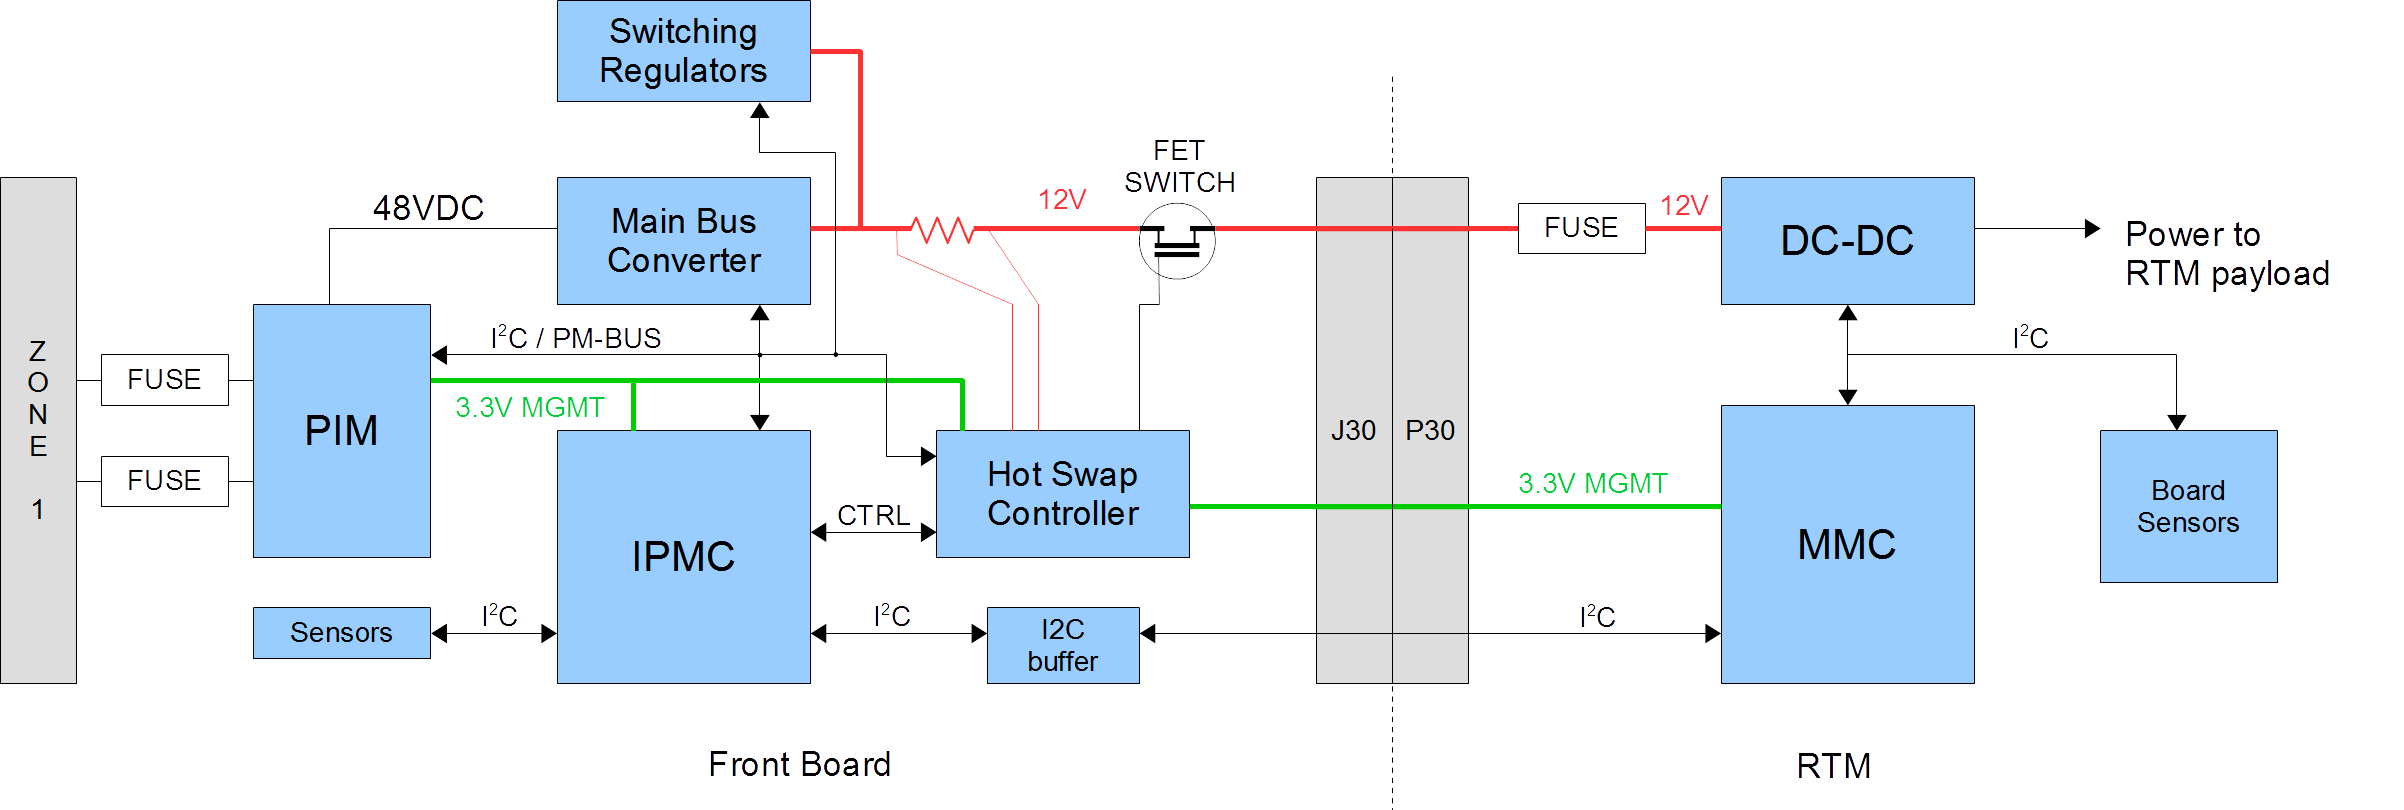
\includegraphics[width=14cm]{rtm_pwr.png}
\caption{Front board and RTM power routing and management connections.}
\label{rtm_pwr}
\end{figure}

The RTM is powered through the J30/P30 connector which mates to the Pulsar IIb front board.  Through this connector 3.3V management power and the main 12V power rails are delivered to the RTM.  Both management and main power rails are monitored and controlled by the IPMC module on the Pulsar IIb front board.  The power and management connections related to the RTM are shown in Figure \ref{rtm_pwr}.

When the RTM is inserted into the shelf the IPMC first enables the 3.3V management power to the RTM.  This allows the RTM MMC microcontroller to boot and begin communication with the IPMC over the I2C bus.  The IPMC collects information about the RTM such as sensor data, number and type of installed transceivers, power requirements, etc.  The IPMC then informs the ShMM that additional sensor data records have been activated and the ShMM adds these records to the list of sensors to scan periodically.  At this point the ShMM informs the IPMC that the RTM main power may be activated.  The IPMC commands the hot swap controller to enable the FET switch thus powering up the RTM payload.

The hot swap controller on the front board constantly monitors the voltage and current supplied to the RTM on the 3.3V management and main 12V power rails.  In the event of an over-current or over-voltage condition the hot swap controller will disable power to the RTM and will set appropriate error status bits, which will be read by the IPMC and passed along to the ShMM.

If the RTM is in an active powered up state the act of opening the RTM lower handle causes the MMC to send a deactivation request message to the IPMC.  The IPMC passes this deactivation message along to the ShMM.  The ShMM then removes any applicable sensor data records from its internal database and responds to the IPMC with a request granted message.  Upon receipt of this message the IPMC commands the hot swap controller to kill the main power to the RTM.  The 3.3V management power to the RTM remains enabled until the RTM is physically unplugged from the front board.

% *****************************************************************************

\section{Intelligent Platform Management Controller}
\label{ipmc_section}

\begin{figure}
\centering
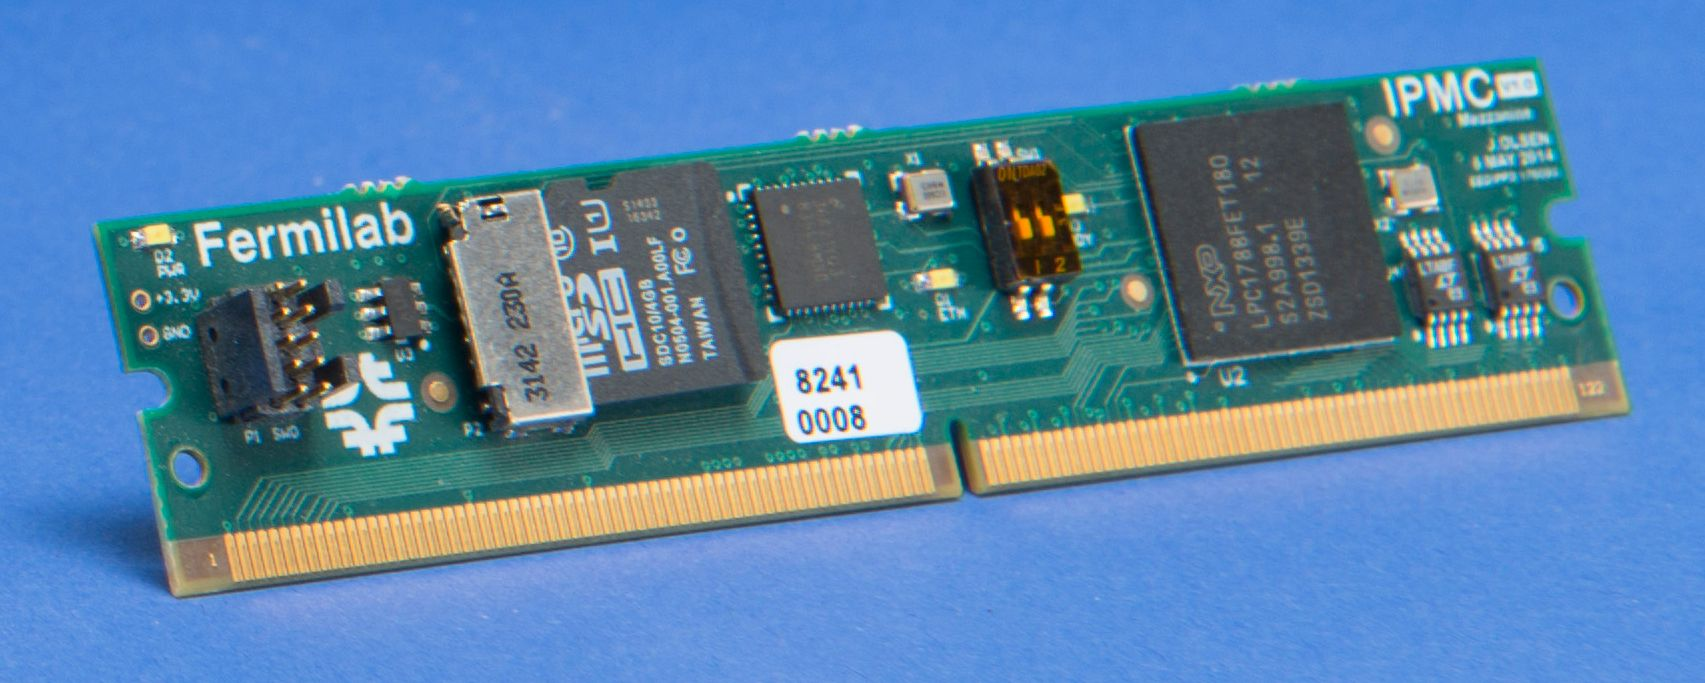
\includegraphics[width=12cm]{fnal_ipmc.jpg}
\caption{The Fermilab IPMC mezzanine card.}
\label{fnal_ipmc}
\end{figure}

A small microcontroller is used as an Intelligent Platform Management Controller (IPMC), which is required on all ATCA boards. This microcontroller is responsible for communicating with the ATCA shelf manager using the Intelligent Platform Management Interface (IPMI).  Through this interface the dual redundant shelf manager boards monitor temperature and other various board sensors, and coordinate hot swap operations, and configure various board functions.

Several different HEP groups have endevored to produce an IPMC mezzannine card \cite{lapp_ipmc}\cite{cern_ipmc}\cite{wisc_ipmc}.  Thankfully all groups have settled upon a common form factor and standardized pinout based on a low profile 244-pin mini DIMM module.  The FNAL IPMC mezzanine shown in Figure \ref{fnal_ipmc} was designed to be simple test platform for implementing basic IPMI functionality as well as some limited extra-IPMI slow control functionality.  The Fermilab IPMC uses an ARM Cortex M3 microcontroller (NXP LPC1788FET180) which has 512kB flash, 96kB RAM, and peripherals such as Ethnet, I2C, SPI, etc.  A lightweight real time operating system (KEIL RTX) is used to manage multiple tasks running concurrently and a Ethernet MAC and TCP/IP network stack.  The LPC Cortex-M3 microcontroller may be programmed only via a direct connection to the 10-pin programming header on the mezzanine.

\subsection{Core IPMI Functionality}

As soon as the Pulsar2b board is installed in a shelf the IPMC boots and begins to communicate with the active shelf manager board over the IPMI I2C interface.  The IPMC identifies itself to the shelf manager, which in turn asks for various Sensor Data Records from the IPMC.  These SDRs contain raw sensor readings, description and threshold bits, which the shelf manager uses to build a board profile.  Once the shelf manager has determined that the Pulsar2b board power requirements and other ``e-key" handshaking has been completed successfully it informs the IPMC that it may turn on power to the board payload (main FPGA, mezzanines).  If the RTM is present, the IPMC communicates with the microcontroller on the RTM and also passes this information back to the shelf manager.  Power to the RTM is controlled by the IPMC.  When the boards are in an operational/active state the shelf manager periodically requests updated SDRs from the IPMC.  If any sensor is above or below threshold the shelf manager may generate a minor, major, or non-recoverable alarm state.  If a Pulsar2b board or FPGA temperature sensor is above threshold the shelf manager will increase the fan speed as well.  The Pulsar2b board contains over 30 various sensors to monitor temperature, voltage, current.

Virtually every component in an ATCA shelf is designed to support hot swap insertion and removal.  To remove an Pulsar2b board or RTM first open the lower handle part way and observe the blue HS LED.  This LED should blink slowly for a moment while the IPMC and shelf manager negotiate the shutdown procedure and deactivate payload power.  Once the HS LED is solid blue the board may be removed from the system.  Note that Pulsar II mezzanine cards are NOT hot swappable and can only be removed when the Pulsar2b has been removed from the shelf.

The IPMI specification is deceptively complex as the query/response transations build in complexity as the shelf manager learns more about the board.  The Fermilab IPMC software was designed from scratch reading through the IPMI and PICMG documentation and also snooping on the traffic between the IPMC and shelf manager.  Complete coverage of the IPMI protocol is not expressly claimed but so far the Fermilab IPMC seems to work fine with the various shelf manager boards in our test stands.

\subsection{Non-IPMI Features for Slow Controls}

The Fermilab IPMC supports a 100Base-T Ethernet interface, which is used for non-IPMI services over TCP/IP.  These services are used for monitoring and various slow controls functions.  The MAC address and static IP address of the Ethernet interface are derived from the IPMI hardware address set on the backplane.  On the Pulsar2b board the Fermilab IPMC Ethernet inteface connects to the backplane Base Interface port number 1 and to the Ethernet switch in logical slot number 1.

\subsubsection{Xilinx Virtual Cable JTAG Interface}

The FNAL IPMC acts as the master on a JTAG bus which connects to the main FPGA and four mezzanine cards on the Pulsar2b board.  One way to program the FPGAs on the boards is to plug in a JTAG cable locally.  Another option is to program the FPGAs over the network using the Xilinx Virtual Cable (XVC) protocol.  The IPMC listens on TCP port 2345 for incoming connections from the Xilinx Vivado Hardware Manager program.  Once Vivado has connected to the Pulsar2b IPMC over the network bitstream files can be programmed into the devices and diagnostics such as chipscope and the serial link analyzer can be run remotely.  The FNAL IPMC XVC implementation is efficient and throughput is roughly equivalent to a local USB JTAG cable.

\subsubsection{SPI Server}

The FNAL IPMC connects to the main FPGA over a simple bidirectional four wire SPI bus.  This bus is designed to sent simple commands and data to and from registers and memory buffers implented in the main FPGA firmware.  To access this bus the user connects to the IPMC over the network on TCP port 1234.  Once connected, enter 64 bits (represented by a string of 16 hex ascii characters) and hit return.  These 64 bits are clocked into the main FPGA on the MOSI line and 64 bits are sampled on the MISO line and returned to the user as a 16 character hex string.  Note that the meaning of these 64 bits is user-defined by the author of the SPI slave module which resides in the main FPGA.  The SPI bus may also be accessed from the telnet command line.

\subsubsection{FTP}

A micro-SD flash memory card is present on the FNAL IPMC and files may be transferred to and from this filesystem over anonymous FTP.  FPGA bitsream files (*.bit and *.xsvf) may be transferred to the filesystem so that FPGAs may be programmed automatically upon powerup.  The IPMC also updates a log file which resides on the flash filesystem.

\subsubsection{Telnet}

Users may also telnet into the IPMC to access slow control functions via a command line.  There is no username or password on this telnet login as this system was designed to operate on a private network.  The command line main menu looks like this:

\begin{verbatim}
Pulsar2b> help

    IPMC User Commands:
    ----------------------------
    fpga  - report FPGA status
    rtm   - report RTM status
    ipmc  - report general module status
    sensor - show sensor readings
    bpclk {0|1} - backplane clock driver
    spi   - read or write to FPGA SPI interface
    bye   - close this telnet session
 \end{verbatim}

Note that the BPCLK command is used to control the backplane synchronization interface.  The Pulsar2b board designated as the shelf clock master must have the M-LVDS driver enabled by typing ``BPCLK 1" at this menu.  The power on default is to DISABLE the M-LVDS driver.  This control is only accessible through this telnet interface.

% *****************************************************************************

\section{Link Performance Testing}
\label{link_perf}

On the Pulsar IIb board the Virtex-7 FPGA is directly connected to the RTM, four FMC mezzanine card slots as well as the ATCA full-mesh backplane fabric.  This direct connection to the enables the full diagnostic capabilities of the MGT transceivers to evaluate the quality of the links at speeds up to 10 Gbps.  

First, some background information about link testing.  The best indicator of the quality of a high speed link channel is a wide open eye diagram, which indicates large signal margins at the receiver.  In the eye diagrams presented in this document the deep blue area represents an operating region where the bit error ratio is better than 10\textsuperscript{-9}.

Historically the eye diagram measurement required the use of a very expensive high speed oscilloscope and very expensive low capacitance active probes.  As serial line rates continued to rise, and as signal amplitudes have continued to drop, direct probing of high speed signals has become challenging.  One reason for this is that even a high quality scope probe adds a few pF of capacitance, and that additional capacitance is highly disruptive and distorts the waveform's fast (~10 picosecond!) edges.  Another reason is that high density high pin count BGA packages and high speed PCB layout techniques generally leave no good places to even probe the signals of interest!

Thankfully, silicon designers have addressed these challenges by building advanced diagnostic features into the transceiver itself.  Unlike direct observation with an oscilloscope, internal monitoring shows what the received signal looks like after termination and equalization stages have been applied.  In Xilinx FPGAs these advanced transceiver diagnostic status and control ports available to the user fabric and JTAG interface.  From the Xilinx Vivado Hardware Manager software users can then tune the transceivers and view the statistical eye diagrams in real time.  The following sections summarize our results from extensive testing of the various high speed interfaces on the Pulsar2b board.

\subsection{Full Mesh Backplane}

The abundance of high speed backplane links makes the Pulsar IIb an ideal test platform for characterizing ATCA backplane performance, and to date several vendors have submitted their latest high performance 14 slot full mesh ATCA backplanes to our group for testing.  Our backplane test results indicate that channel performance consistency is one of the most significant challenges facing ATCA backplane manufacturers today.  

\subsubsection{10G and 40G Backplane Testing}
\label{link_perf_40g}

\begin{figure}
\centering
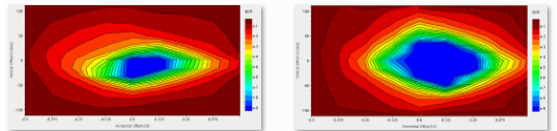
\includegraphics[width=12cm]{bad_links.png}
\caption{Inconsistant link performance on an early 40G backplane.}
\label{bad_links}
\end{figure}

Full mesh ATCA backplane testing at Fermilab involves loading several Pulsar2 boards into a shelf, then loading the FPGAs with Xilinx IBERT link test firmware.  This firmware drives data patterns out on all backplane TX channels and provides the user with full diagnostic features on the receive side.  Through the JTAG interface the Xilinx Vivado Hardware Manager software enables full control of the MGT TX and RX tuning parameters.

Our first experiences with a full mesh backplane were encouraging.  The test shelf featured a full mesh backplane  rated for 10G per channel (that is, four lanes at 2.5Gbps).  The backplane manufacturer indicated that the maximum line rate we should expect would be in the range of 3 to 4Gbps per lane.  Our testing however revealed acceptable performance at 6.6Gbps per lane (the limit of our first ATCA board design, the Pulsar2a) with minimal transceiver tuning.  When our Pulsar2a boards were installed in a newer shelf with a 40G backplane the link margins and eye diagrams looked even better at 6.6Gbps.

The Pulsar2b board enabled backplane testing to continue at line rates up to 10Gbps per lane.  At speeds above 6.6Gbps the test results were however inconsistent and more difficult to interpret.  Several different 40G backplanes from multiple vendors were evaluated in our test stand at Fermilab.  Within a shelf a the backplane link performance between pair of Pulsar2b boards would vary significantly from slot to slot.  Some slots had beautiful wide open eye diagrams while other slots struggled to establish a link at all or suffered from high bit error rates (Figure \ref{bad_links}.  On some backplanes it was noted that removing and reinserting the Pulsar2b in the same slot led to differences in link performance, which suggests subtle mechanical mis-alignment between the shelf chassis, backplane, and Pulsar2b board connectors.  In all cases our results were shared with the shelf and backplane manufacturers who loaned us the hardware to test.

\subsubsection{100G Backplane Testing}
\label{link_perf_100g}

\begin{figure}
\centering
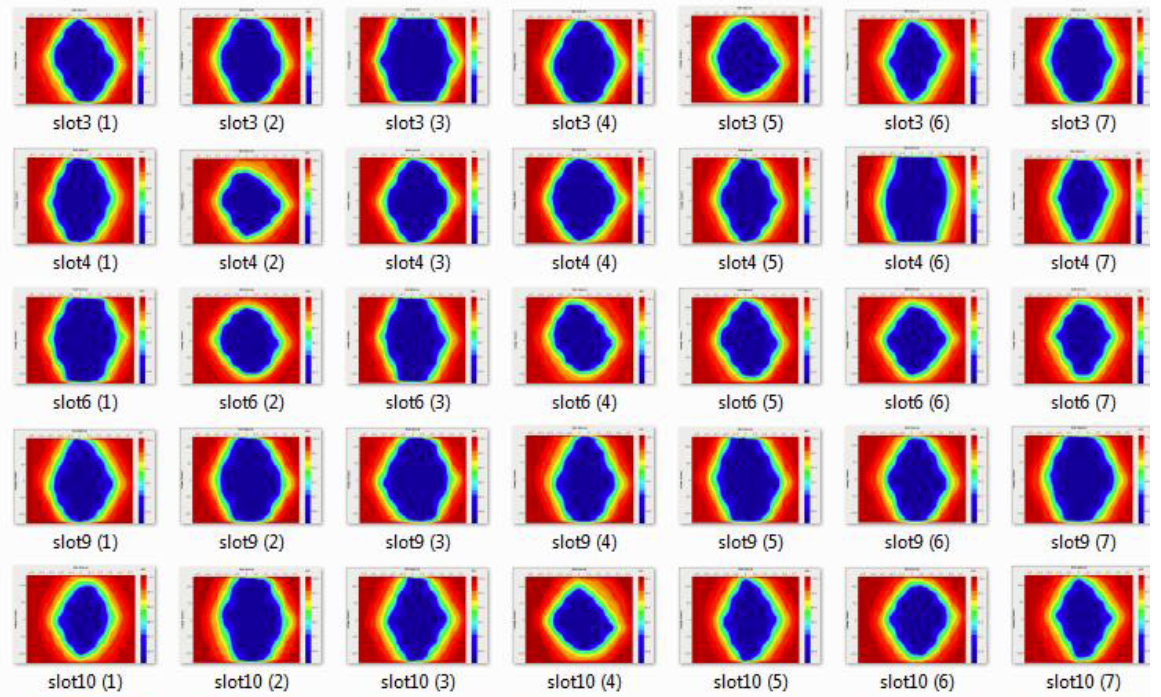
\includegraphics[width=12cm]{comtel_results.png}
\caption{Example links on the COMTEL full mesh backplane, 10Gbps PRBS7.}
\label{comtel_results}
\end{figure}

In 2014 COMTEL delivered to us one of their first prototype ``Air-/-Plane" 100G full mesh backplanes\cite{comtel}.  This backplane was designed with the latest low loss PCB materials and carefully designed to minimize crosstalk and impedance discontinuities through the connectors.  COMTEL internal testing with signal generators and time-domain reflectometer equipment indicated good link performance up to 25Gbps per lane. The engineers at COMTEL were anxious to see ``real world" test results and our Pulsar2b board was the only platform capable of exercising many backplane links simultaneiously.  With this new backplane design the Pulsar2b board performed very well, and for the first time we observed consistantly wide open eyes and error free operation at 10Gbps across the entire shelf as shown in Figure \ref{comtel_results}.  

Now with a high quality backplane we have established that the Pulsar2b board design meets the desgin target of 10Gbps across the backplane.  We suspect that 10Gbps is close to the upper speed limit determined largely by the (legacy ADF/ZD) connectors and PCB materials used on the Pulsar2b board design.  Future Pulsar boards will be based on Xilinx UltraScale FPGAs, improved connectors, and higher performance low loss PCB materials.  These next generation Pulsar boards will seek to demonstrate backplane data rates in the 16Gbps to 25Gbps regime.

\subsection{Rear Transition Module}
\label{link_perf_rtm}

Compared to the longest distance across the ATCA backplane, the traces from the Pulsar2b FPGA to the QSFP+ transceivers on the RTM are short.  When Pulsar2b boards communicate over the full mesh backplane both link endpoints are FPGAs, which means that we have full control over the transceiver tuning parameters on both ends of the link.  However when the Pulsar2b FPGA communicates with a transceiver on the RTM the tuning options are limited by the QSFP+ module copper interface.  Very few QSFP+ modules support advanced controls such as RX equalization, TX output swing, and TX pre-emphasis.  The Pulsar2b FPGA can only adjust the shape and amplitude of the signals going to the QSFP+ transciever.  Likewise, the Pulsar2b FPGA can only adjust the termination parameters and equalization on the signals coming from the QSFP+ transceiver.  With the help of a passive QSFP loopback module we can nevertheless tune the FPGA transceiver parameters to achieve fair results on the 40 RTM links, as shown in Figure \ref{rtm_results}.

Only one manufacturer produces the right angle male ADF/ZD data connector detailed in the PICMG 3.8 RTM specification.  Our test results indicate that at 10GBps this connector performance is marginal.  In particular we have observed crosstalk between adjecent RX TX pairs leading to a reduction in the eye size and bit errors.  Careful tuning can eliminate bit error rates however we are considering using alternative high performance low crosstalk connectors for future RTM and Pulsar board designs.

\begin{figure}
\centering
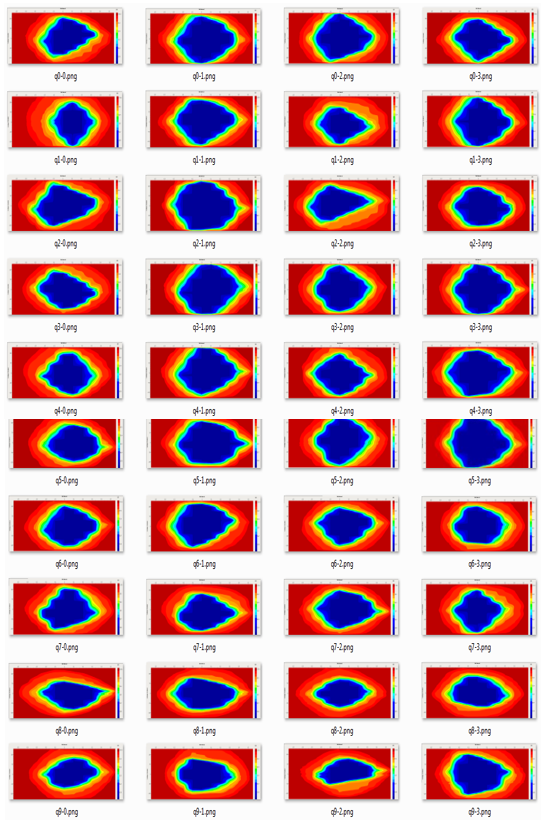
\includegraphics[width=10cm]{rtm_results.png}
\caption{RTM link performance, AOC loopback at 10Gbps PRBS7.}
\label{rtm_results}
\end{figure}

\subsection{Mezzanine Cards}
\label{link_perf_fmc}

The Pulsar2b FPGA connects to four FMC mezzanine connectors, each with 34 user-defined unidirectional LVDS pairs and three bidirectional high speed MGT lanes.  The mezzanine card interface was tested using a passive FMC loopback card as well as a fully functional mezzanine card with a Kintex UltraScale FPGA installed.  For more details about the FMC mezzanine card refer to Fermilab Technical Memo 2651-E\cite{tm2651e}.

\subsubsection{Serial Interface}

A total of 12 GTH transceivers are used for high speed communication between the Pulsar2b FPGA and the FMC mezzanine cards.  Per the VITA 57.1 specification the AC coupling capacitors for these high speed links are to be located on the FMC mezzanine.  Figure \ref{fmc_results} shows 12 eye diagrams depicting the performance of six 10Gbps links between the Pulsar2b FPGA and a Kintex UltraScale KU060-2 device mounted on a double-wide mezzanine card.

\begin{figure}
\centering
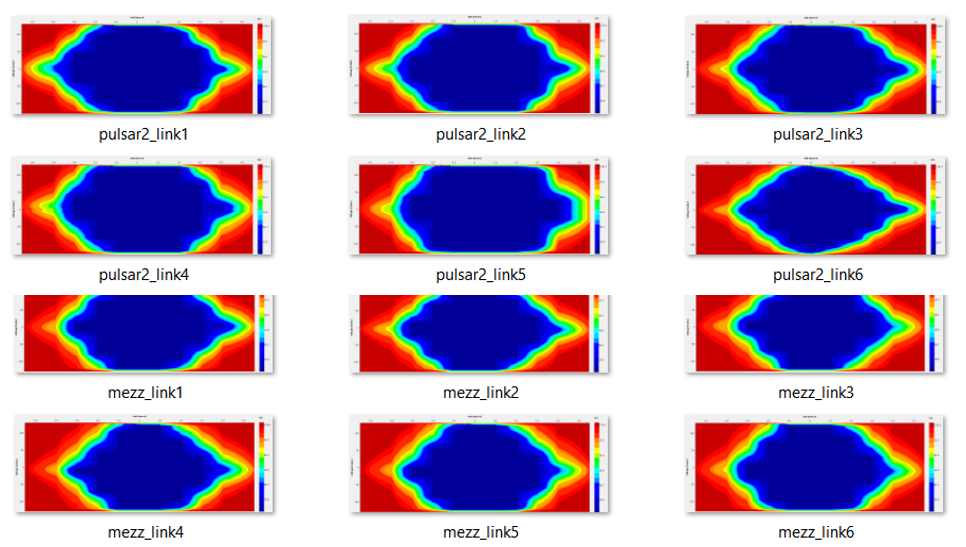
\includegraphics[width=10cm]{fmc_results.png}
\caption{Link performance at 10Gbps PRBS7 between the Pulsar2b FPGA a Kintex UltraScale FPGA on Mezzanine card.}
\label{fmc_results}
\end{figure}

\subsubsection{Parallel Interface}

Unlike the high speed serial lines which embed the clock in the data steam, data transmission over a parallel bus uses a separate clock, and therefore the receivers are sensitive to the timing skew between the data pairs and the clock.  Ideally the clock edges should fall in the center of the data bit valid window as measured at the receiver inputs.  As clock frequencies increase the minimum setup and hold time requirements become a significant portion of the bit period.  Excessive skew on the data lines results in setup and hold time violations which can lead to bit errors.  In our experience the minimum setup and hold times are met using static timing constraints if the clock frequency is less than about 100MHz.  At clock frequencies above 100MHz active deskewing the data lines is required.  Data deskew and realignment is performed by a programmable precision delay line on each I/O pin.  Link training is the process by which the FPGA LVDS receivers adjust this delay line back and forth until the center of the bit period is found.  Once the delay line is set the FPGA then adjusts this calibrated delay line to compensate for voltage and temperature variations.  Using the link training technique we have successfully tested the mezzanine card parallel bus interface up to 800Mbps per LVDS pair (400MHz clock double data rate sampling on the rising/falling edges).  If the mezzanine card or Pulsar2b FPGA is reset the link training procedure should be repeated.

% *****************************************************************************

\section{System Integration}

System integration testing involves not only sending data between Pulsar IIb boards over the backplane channels, but also incorporating the Inter-shelf and Intra-shelf synchronization. In this section we will present the Pulsar IIb hardware and its performance, our two full-crate integration tests including the Inter-shelf and Intra-shelf synchronization using CMS trigger framework control hardware, the results of our 40G and 100G ATCA full mesh backplane performance tests, and how the backplane is used for the development of low-latency time-multiplexed data transfer schemes. Today the Pulsar IIb serial links, including interfacing with RTM and FMC mezzanine as well as full-mesh backplane, all operate reliably at 10 Gbps.  We must nevertheless continue to refine our layout techniques as FPGA transceivers and ATCA backplanes continue their evolution towards ever higher serial bit rates. We will discuss how the push towards higher serial bit rates has challenged us to focus on signal integrity at the PCB level, and the experiences gained throughout the process. 

\subsection{Synchronization}
\label{section_ttc}

As will be illustrated in the following sections it is important to distribute a common clock and control signals all Pulsar2b boards in the system.  

In our test stand at Fermilab we use a TTC optical link\cite{cern_ttc} to synchonize up to 24 Pulsar2b boards in two ATCA shelves.  A CERN TTCcx VME board drives a local TTC optical link that encodes a simulated 40MHz bunch crossing clock and various control signals.  This optical link is passively split and terminates on a pair of custom FMC mezzanine cards.  These FMC cards convert the optical signal into an 80Mbps LVDS data stream and 160MHz LVDS clock.  Firmware in the Pulsar2b FPGA decodes the data stream into a 40MHz bunch crossing clock and control bits, driven out on the backplane as CLK3A and CLK3B respectively.  All Pulsar2b boards in the shelf receive the CLK3A and CLK3B signals from the backplane.  The 40MHz CLK3A clock feeds into a PLL and multiplied up to 240MHz and used as the master clock in the Pulsar2b FPGA.  The control bits encoded on the CLK3B line are demuxed into A and B channels per the CERN TTC specification.  Channel A is used exclusively for the L1ACCEPT control bit, while channel B is used for broadcast control bits such as the bunch crossing zero (BC0) marker and various resets.  (The TTC channel B protocol allows for directed control messages to specific geometric regions of the experiment, however the Pulsar2b synchroniziation  firmware ignores these messages for the time being.)

It is not critical that the synchonization interface distributes a perfectly clean low jitter reference clock to the Pulsar2b boards.  Also, slight timing skew differences between Pulsar2b boards are not a big deal. The main point of the synchronization interface is to keep the Pulsar2b FPGA master clocks frequency locked to a common source and to provide a mechanism to synchronize to the beam turn/orbit structure.  Data transmission between Pulsar2b boards always occurs over high speed serial MGT lines.  Due to the way have configured our MGT transceivers we can make no assumptions about the phase of the recovered clock and must consider each MGT receiver as a separate clock domain.  Our data link transmission scheme runs the high speed links \emph{asynchronously} with respect to the accelerator clock.  FIFOs are used to safely cross between the link clock domains and the master clock domain in each Pulsar2b FPGA, as we will see in the following sections.

\subsection{Serial Link Encoding}

In Xilinx FPGAs the MGTs natively support 8b/10b encoding, and we have used a four byte or 32b/40b configuration at line rates up to 10Gbps.  This older encoding scheme has relatively high overhead, but on the plus side DC line balance is strictly maintained and the number of consecutive 1's and 0's is limited to just a few bits.  (The PRBS7 test pattern is used to model 8b/10b encoded links.)

The serial transceivers also support 64b/66b encoding by performing some of the scrambling and framing operations outside the MGT in the FPGA fabric.  This encoding scheme is more efficient due to the lower overhead however the additional logic increases link latency over 8b/10b native encoding.  Unlike 8b/10b the 64b/66b encoding does not inforce strict DC balance on the data stream, resulting in longer runs of 1's and 0's and the subsequent DC baseline wander tends to shrink the eye pattern.  (The PRBS31 test pattern is used to model 64b/66b encoded links.)

\subsection{Serial Link Clocking and Alignment}
\label{linkclocking}

High speed data transmission between FPGAs must be reliable, robust, and should incur a minimal latency penalty.  In order to minimize latency over the link certain MGT features such as elastic buffers and clock correction have been bypassed or disabled.  The link itself runs asynchronous to the FPGA master clock and FIFOs are used to cross clock domains on both the TX and RX side of the link.  A key point here is that the link data rate is slightly higher than the user data rate, and this insures that the number of words stored in the FIFOs is kept to a minimum, as this directly impacts link latency.

\begin{figure}
\centering
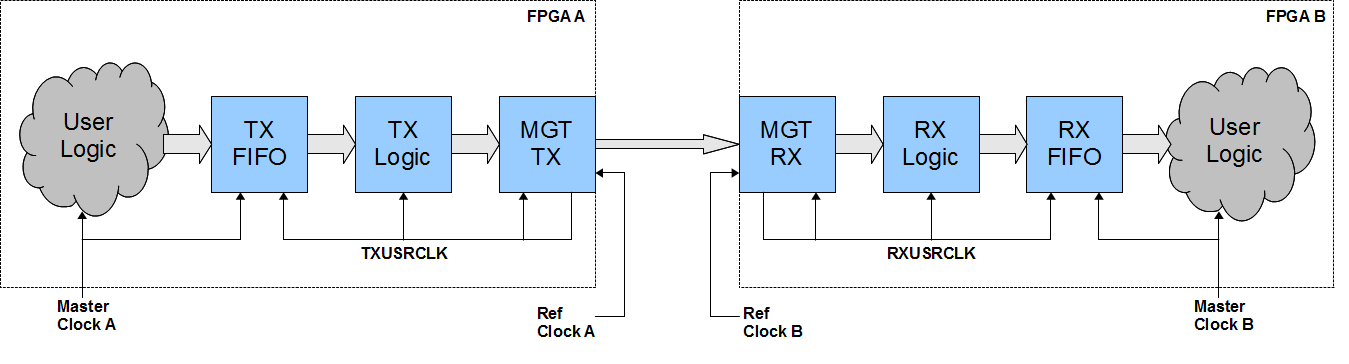
\includegraphics[width=15cm]{link_cdc.png}
\caption{High speed serial link clock domain crossing and data alignment scheme.}
\label{link_cdc}
\end{figure}

Figure \ref{link_cdc} shows two FPGAs located on different boards.  The phase relationship between Master Clock A and Master Clock B is unknown, however these clocks are frequency locked as they are derived from a common source (e.g. the bunch crossing clock) which is distributed over the backplane.  Reference clocks A an B are very close in frequency, but not exactly matched as they are derived from local low jitter oscillators on the two boards.  TXUSRCLK is derived from reference clock A.  RXUSRCLK is derived from the clock recovered from the incoming data stream.  (Note that reference clock B is used only to assist the RX MGT PLL lock onto the incoming data stream. RXUSRCLK is not related to reference clock B.)

On the transmit side the user logic writes into the FIFO on the master clock domain.  The TX LOGIC block looks at the TX FIFO status flags.  If the TX FIFO is not empty then a data word is read from the FIFO, encoded, and sent over the link.  If the TX FIFO is empty the TX LOGIC sends a synchronization word such as a K28.5 commas (8b/10b) or command word (64b/66b).  These special synchronization words must be sent periodically to insure that the MGT RX properly determines the word boundaries on the incoming serial data.  Under normal operating conditions the TX FIFO will periodically go empty since TXUSRCLK is faster than Master Clock A.

On the receive side the MGT RX block deserializes the data stream and outputs parallel words, usually 64 or 32 bits wide.  RX LOGIC block discards the synchronization words and writes all other data words into the RX FIFO.  The RX user logic waits for the RX FIFO to go non empty, and then begins to read from the RX FIFO in the Master Clock B domain.

This link synchronization scheme has been demonstratred with GTH transceivers in 7-series and Kintex Ultrascale devices at line rates up to 10Gbps.  Total link latency varies from 100ns (with 8b/10b encoding) to 150ns (with 64b/66b encoding).

% ***************************************************************************************************************

\section{The CMS L1 Tracking Trigger Demonstration System}

\subsection{Introduction}

To say that the L1 tracking trigger at CMS is challenging hardware project is an understatement.  The CMS detector  inner tracker consists of over 13,000 silicon modules arranged in barrels and disks.  Each front end silicon module outputs the coordinates of the hits (aka stubs) it detects in each 25ns bunch crossing; this translates into a average continuous data rate on the order of ~7Gbps per module, or ~100Tbps for the entire tracker.  As a level-1 system the tracking trigger must observe every bunch crossing and within a few microseconds reconstruct particle tracks, tagging ``interesting" events for more detailed reconstruction and analysis performed by downstream trigger systems and offline CPU farms.  

The extremely high input data rate and tight latency requirements dictate that the tracking trigger is implmented as a massively-parallel, hardware-based, brute-force pattern recognition engine.  In our demonstration system the pattern recognition stage uses a combination of FPGAs and Pattern Recognition Associative Memory (PRAM)\cite{pram} custom ASIC chips; this logic is located on a small board we call the Pattern Recognition Mezzanine (PRM) and is described in detail in Fermilab Technical Memo 2651-E\cite{tm2651e}.  

Designing the high performance PRM is however only one challenging part of the demonstration system.  Another formidible challenge is data delivery, or the mechanism by which the input stubs are routed from the front end detector modules to the PRMs.  The data delivery challenge is partially physical, that is, how should the detector be partitioned and how should fibers be routed between boards in an manner that is efficent, scalable, and flexible.  The other part of the data delivery challenge all about buying time.  At the LHC each bunch crossing is 25ns and that event rate is simply too fast for a single PRM to process an event.  It's not even enough time to get any meaningful work done in a single pipeline stage.  So the way we extend or create more processing time is to use several PRMs in parallel and use time multiplexed data transfers to distribute event data.  In order to tackle the data delivery challenge we divide and conquer in both space (by dividing the tracker into regions or towers) and time (by time multiplexed data transfers).  In the following sections we show how the Pulsar2b front boards and the ATCA full mesh backplane address the data delivery challenge and offer a solution that is elegent, balanced and flexible.

\subsection{Data Delivery Overview}

The L1 Tracking Trigger demonstrator is designed to model one trigger tower, or a region of the detector consisting of approximately 290 front end modules.  In order to find tracks which originate in neighboring towers the front end module data is duplicated and shared across tower boundaries and this increases the number of links by 10\%, for a total of 320 links per tower.  The trigger tower processor is a single 14-slot ATCA shelf with up to 12 Pulsar2b boards, which are configured to be Pattern Recognition Boards (PRB). Typically we use 10 PRBs per shelf, which is a managable 32 input links per board.

In the following sections we will illustrate how the PRB boards in shelf communiate with each other over the full mesh backplane.  This new architecture is unique in that it effectively blurs the distinction between individual PRBs; one benefit of the robust interconnections between PRBs is that a fiber may enter the shelf on \emph{any} input.  When one considers all inputs to be equivalent this opens up options for link balancing, load sharing, future expansion, redundancy, etc.  The full mesh architecture is compared and contrasted with more traditional, fixed ``direct flow" interconnections in Appendix \ref{Appendix_DirectFlow}.

All PRBs in the shelf receive module data over the fiber links.  Stubs (aka hits) for 8 events (aka bunch crossings, BX) are packed into 200ns fixed length packet or ``train".  This format allows for some variation in the number of stubs per BX. Trains are roughly aligned in time (to within a nanosecond or so) and are received continously with no inter-train gaps.

As mentioned previously, each BX is only 25ns.  This period is too short to perform any real processing of event data.  Time multiplexing event data an array of identical processors is the technique we employ to increase the amount of time between events.  The process by which PRB boards receive input data, exchange data over the backplane, and present the stubs for a complete BX to a PRM mezzanine is what we refer to as \emph{data delivery}.  In our demonstration system we use time muliplexing period of 20, which means that a given PRM will see every 20th event (or a new event every 500ns). It's worth pointing out that the PRM cannot do ALL the processing within 500ns; within the PRM the processing stages are still pipelined and thus at any given time there are several events working their way through the PRM.  Time muliplexing increases the maximum time we can take in each pipeline stage.  For example, we have 500ns to transfer all stubs from the PRB up to the PRM mezzanine; we have 500ns to transfer stubs into the PRAM device; we have 500ns to read out the roads from the PRAM, etc.

\subsection{Fermilab Test Stand}

\begin{figure}
\centering
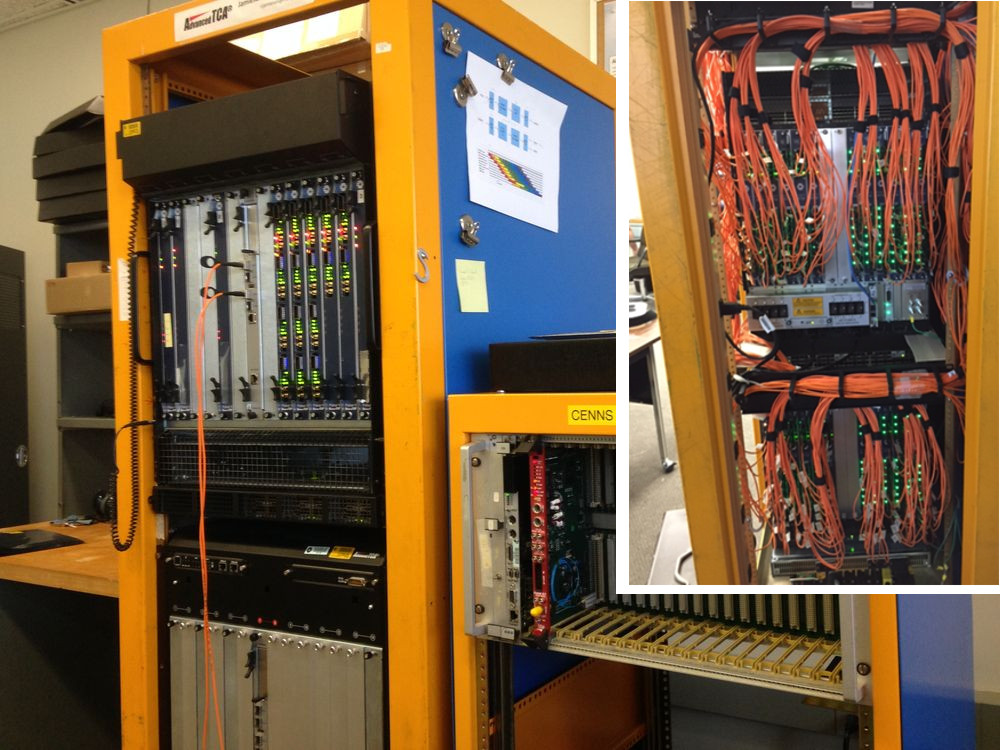
\includegraphics[width=12cm]{teststand.jpg}
\caption{The Pulsar2 test stand at Fermilab.  The upper ATCA shelf (COMTEL) is for Pattern Recognition Boards (PRBs) and the lower shelf (Schroff) is for Data Source Boards (DSBs).  The short rack contains a VME crate and TTCcx board.  Inset: the rear of the rack showing 100 QSFP+ cables connecting the two ATCA shelves.}
\label{teststand_pic}
\end{figure}

Our tracking trigger test stand is comprised of two ATCA shelves and a VME crate shown in Figure \ref{teststand_pic}.  The VME crate hosts the TTCcx board, which drives the master clock and control signal on a short optical fiber to the two ATCA shelves.  Ten Pulsar2b boards in the lower ATCA shelf are configured as Data Source Boards (DSB).  These DSBs do not have any mezzanine cards installed and require no communicatation across the full mesh backplane.  Test vectors are loaded into the DSBs and then sent at high speed (up to 10Gbps) through 100 QSFP+ fibers to ten Pulsar2b boards in upper ATCA shelf.  The upper ATCA shelf is the ``device under test" where the Pulsar2b boards are configured as Pattern Recognition Boards (PRB).  In this shelf the PRBs communicate over the full mesh backplane to implement the time multiplexed data transfer scheme.  A few PRBs in this shelf have PRM mezzanines installed which allows us to test the full chain from input stubs to found tracks.

\subsubsection{Safety and Interlocks}

\begin{figure}
\centering
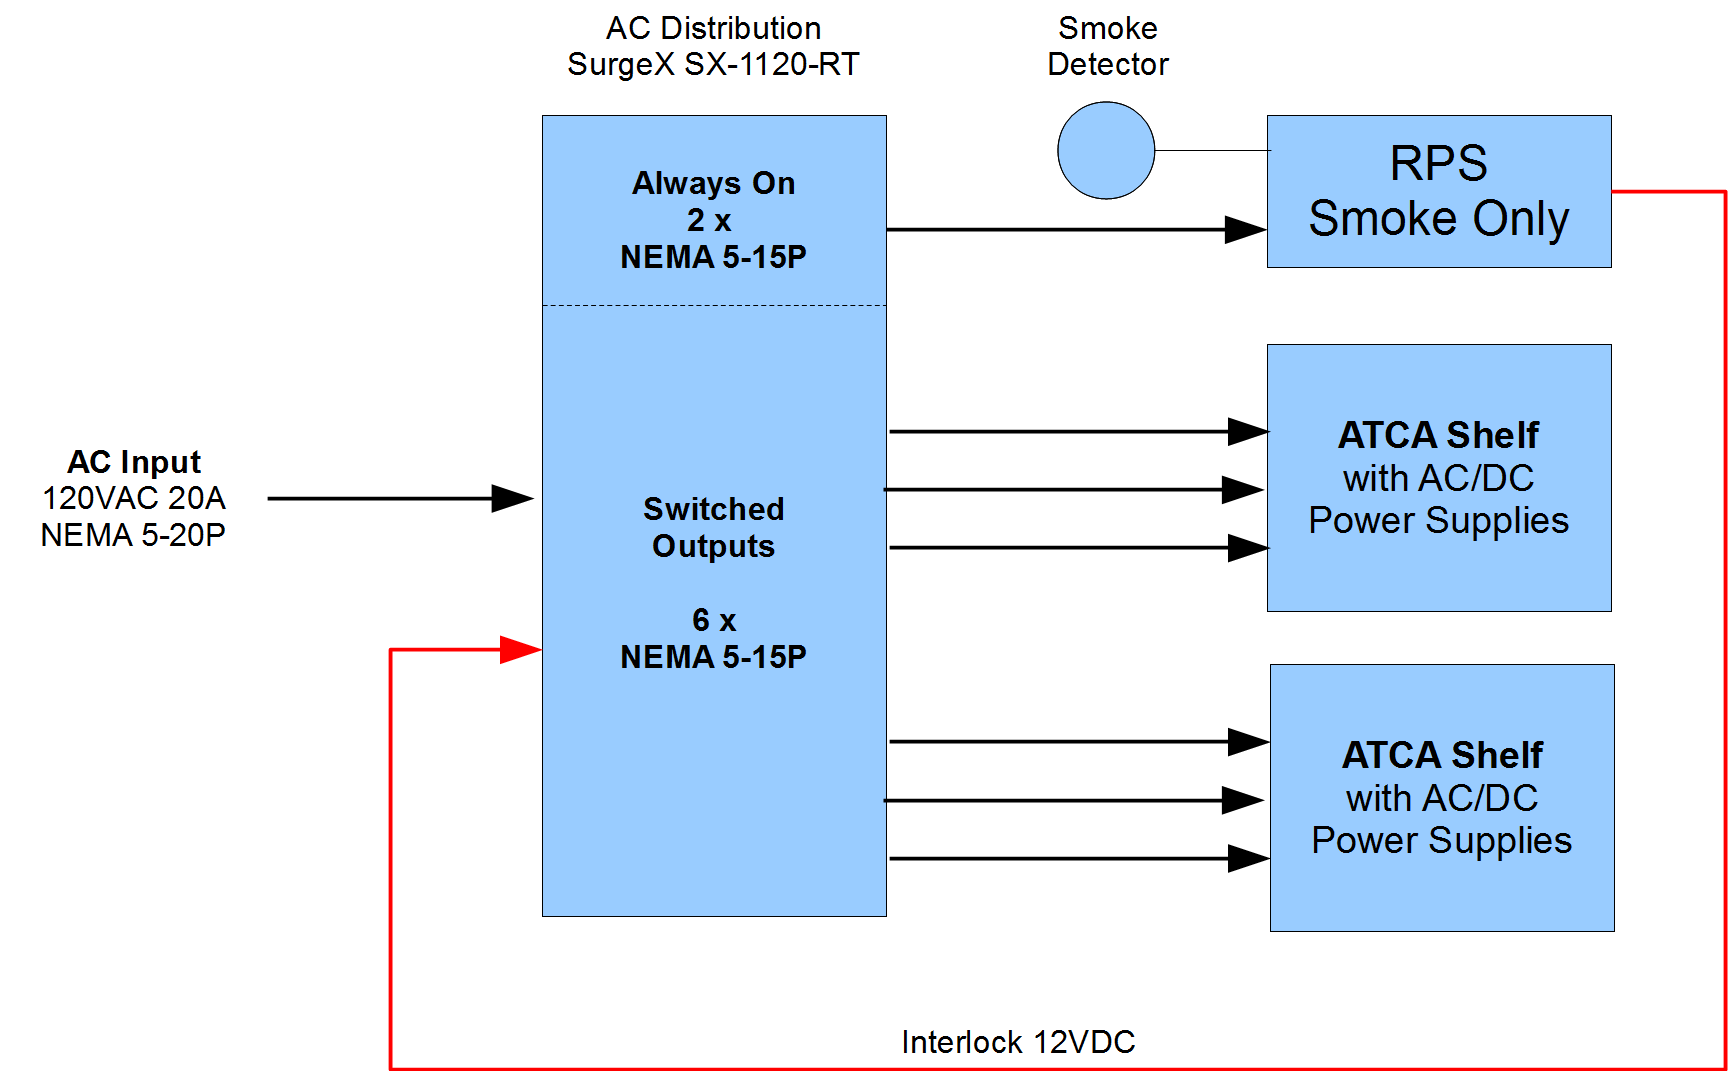
\includegraphics[width=12cm]{interlock.png}
\caption{Smoke detection and AC power interlock in the test stand rack.}
\label{interlock}
\end{figure}

The rack is fitted with a smoke detector and AC power interlock system as shown in Figure \ref{interlock}.  A single phase 20A 120VAC outlet is sufficient for powering the rack.  If smoke is detected the Rack Protection System (RPS) 1U chassis \cite{rps} will drop the 12VDC interlock signal and the AC distribution system (SurgeX SX-1120-RT) will cut power to the two ATCA shelves in the rack.  AC power will remain off and the RPS  will sound an alarm until manually reset.  The upper ATCA shelf is a COMTEL CO-14 chassis with up to five redundant AC/DC power supplies; currently we are only using 3 power supplies in this shelf.  The lower ATCA shelf is a Schroff/Pentair 40G model with a single AC-DC power supply installed (three PS bays are empty).

\subsection{Data Source Boards}

% this is a generic simple version put together by JTO, Lucas and Vitor can update it

The DSB stores simulated event data in a TX buffer and injects this data into the system at full speed.  DSBs can also receive link data at full speed and store it in RX buffers for later readout.  In our test stand we use 10 Pulsar2b boards as DSBs and these boards send and receive up to 400 links at rates up to 10Gbps for a total of 4Tbps.  This is enough links to simulate inputs coming from front end modules in the home tower and a portion of each neighbor tower as well.  DSBs are synchronized to the master clock and support continuous and one shot burst transmission modes.  Event data is stored in the internal buffers in the DSB FPGA and this memory is deep enough to hold several hundred events.  These event data buffers may be written to or read at any time from a Linux PC on our local network.  

\subsubsection{DSB Firmware}

\begin{figure}
\centering
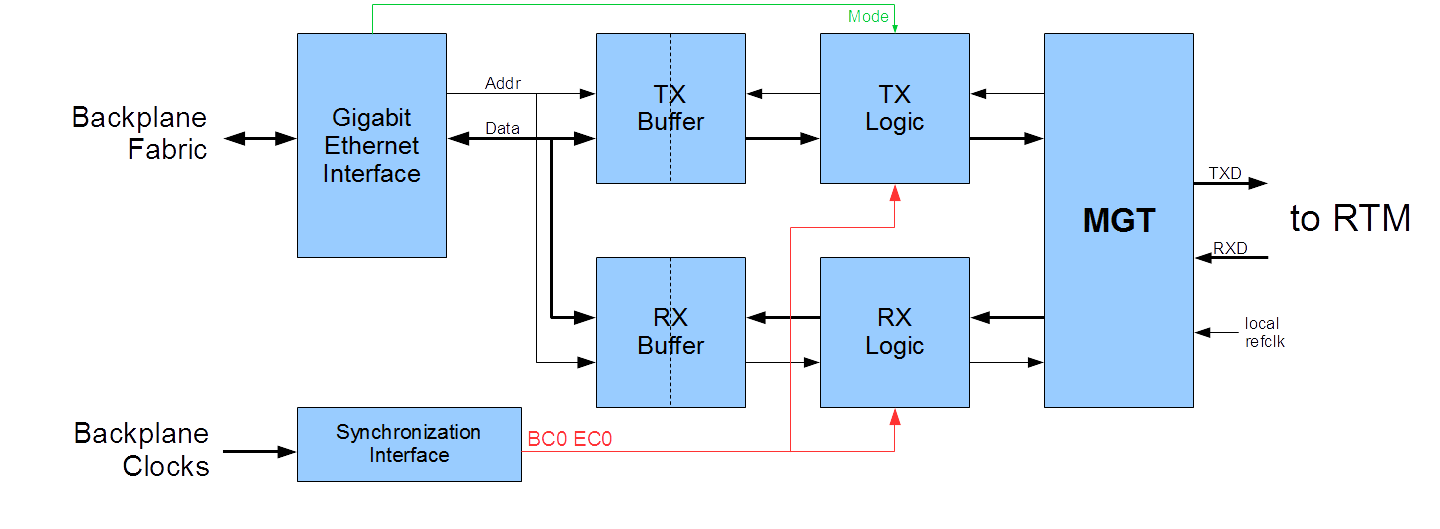
\includegraphics[width=15cm]{dsb.png}
\caption{Data Source Board firmware block diagram.}
\label{dsb_fw}
\end{figure}

A simplified version of the DSB firmware is shown in Figure \ref{dsb_fw}. 

The synchronization interface receives the TTC CLK3A and CLK3B signals from the ATCA backplane as described in Sections \ref{section_bp_sync} and Section \ref{section_ttc}.  From these TTC signals the synchronization interface firmware extracts a bunch crossing zero (BC0) signal which indicates the first BX of an LHC orbit (period = ~89 microseconds) and event counter reset signal (EC0) which is a generated by the the user.

The TX Logic module operates in either single shot or continuous mode.  In single shot mode this module waits to be armed by the the user asserting EC0.  Then, at the next BC0 the TX Logic begins to dump the contents of the TX Buffer to the MGT transmitter.  When the end of the TX Buffer is reached it then halts and waits to be re-armed by EC0.  When idle the MGT transmitter sends nulls or comma characters.  In continous mode the TX Logic automatically re-arms at the end of each LHC orbit, so that the first word of the TX Buffer always follows shortly after BC0.  The TX Logic and TX Buffer are clocked by the MGT TXUSRCLK, which is derived from the local reference clock oscillator.  To the TX Logic module the BC0 and EC0 signals are \emph{asynchronous}, and therefore sampling error will result in link to link skew of one TXUSRCLK period (worst case a few nanoseconds).  This is not a problem for the reasons described in Section \ref{linkclocking}.

On the receive side the RX logic module waits to be armed by the user asserting EC0.  Once armed the RX Logic module waits for the BC0 marker then stores the next N words it receives from the MGT.  The contents of the RX buffer may then be read out through the Ethernet interface.  The RX Logic module and RX Buffer are clocked by the RXUSRCLK from the MGT.

\subsubsection{DSB Network Connection}

The Gigabit Ethernet Interface allows users read and write access to the TX and RX Buffers; these buffers are implemented in dual port BlockRAM and may accessed at any time.  In the DSB firmware the Ethernet interface has been implemented using the IPBus\cite{ipbus} and ``Off the shelf" Ethernet interface (OEI)\cite{oei} firmware designs.  Both interfaces use a simple UDP packet protocol to perform block writes and reads to and from addresses defined in the DSB firmware. The DSB board uses backplane fabric channel 1 port 0 to establish a full duplex gigabit Ethernet link to a switch in logical slot 1.   A Linux PC connects to this ATCA switch forming a private network used to communicate with the DSBs in the shelf.

\subsection{Pattern Recognition Boards}
\label{section_prb}

\begin{figure}
\centering
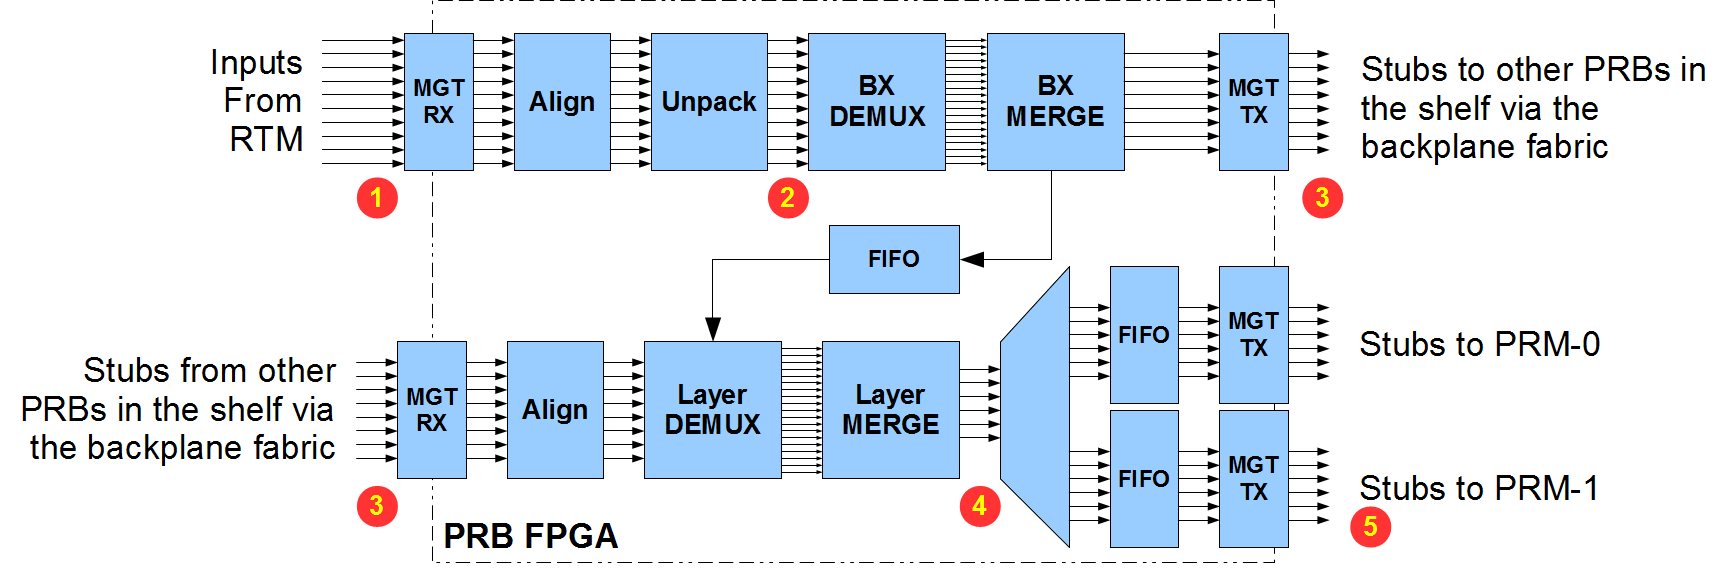
\includegraphics[width=15cm]{prb.png}
\caption{The Pattern Recognition Board firmware block diagram.  The observation points shown in red are used to describe PRB latency figures in Section \ref{section_latency}.}
\label{prb_fw}
\end{figure}

The primary function of the PRB is data delivery: to receive stubs on the RTM inputs; to unpack and sort stubs by BX; to exchange stubs with other PRBs over the full mesh fabric backplane; to sort stubs by layer; and finally, to deliver the complete set of stubs for one BX to a PRM mezzanine.  At all stages the PRM firmware has been optimized to reduce latency to a minimum.  

It's important to note that most stubs entering the shelf will pass through TWO PRB FPGAs before arriving at the destination PRM.  First, stubs arrive at the RTM input and are aligned, unpacked, demultiplexed by BX, and merged before being sent over the backplane to another PRBs. Secondly, stubs enter the PRB FPGA from the backplane and these stubs are then aligned, demultiplexed by layer and merged into a few streams before transmission to the PRMs.  If an incoming stub (from the RTM) does not need to be shared with any other PRB in the shelf it bypasses the backplane completely and is stored in a FIFO used directly to the second stage layer sort logic as shown in Figure \ref{prb_fw}.

\subsubsection {Receive Logic, Alignment and Unpacking}

The PRB FPGA receives up to 40 links from the RTM.  Deskewing and aligning these data streams is described in Section \ref{linkclocking}.  Both 64b/66b and 8b/10b encoding standards have been used in the PRB firmware designs; the MGT data bus width is however 32 bits regardless of 
the encoding standard employed.

The input packet or ``train" format has a fixed length of 200ns and trains arrive continuously with no gaps in between.  Each ``PRBF1" format train consists of: header; a trailer; and payload section with a variable number of stubs for 8 BX.  Unfortunately in this format specification the stub word boundaries do not align with the 32 bit MGT data bus.  This means that the entire 200ns train must be unpacked by first shifting the data into FPGA registers and then copied over to another set of registers before reading out.  After the unpacking stage stubs are aligned to internal 32 bit buses and are transferred on a single clock edge.

\subsubsection {BX Demux and Merge Logic}
\label{merge_logic_section}

\begin{figure}
\centering
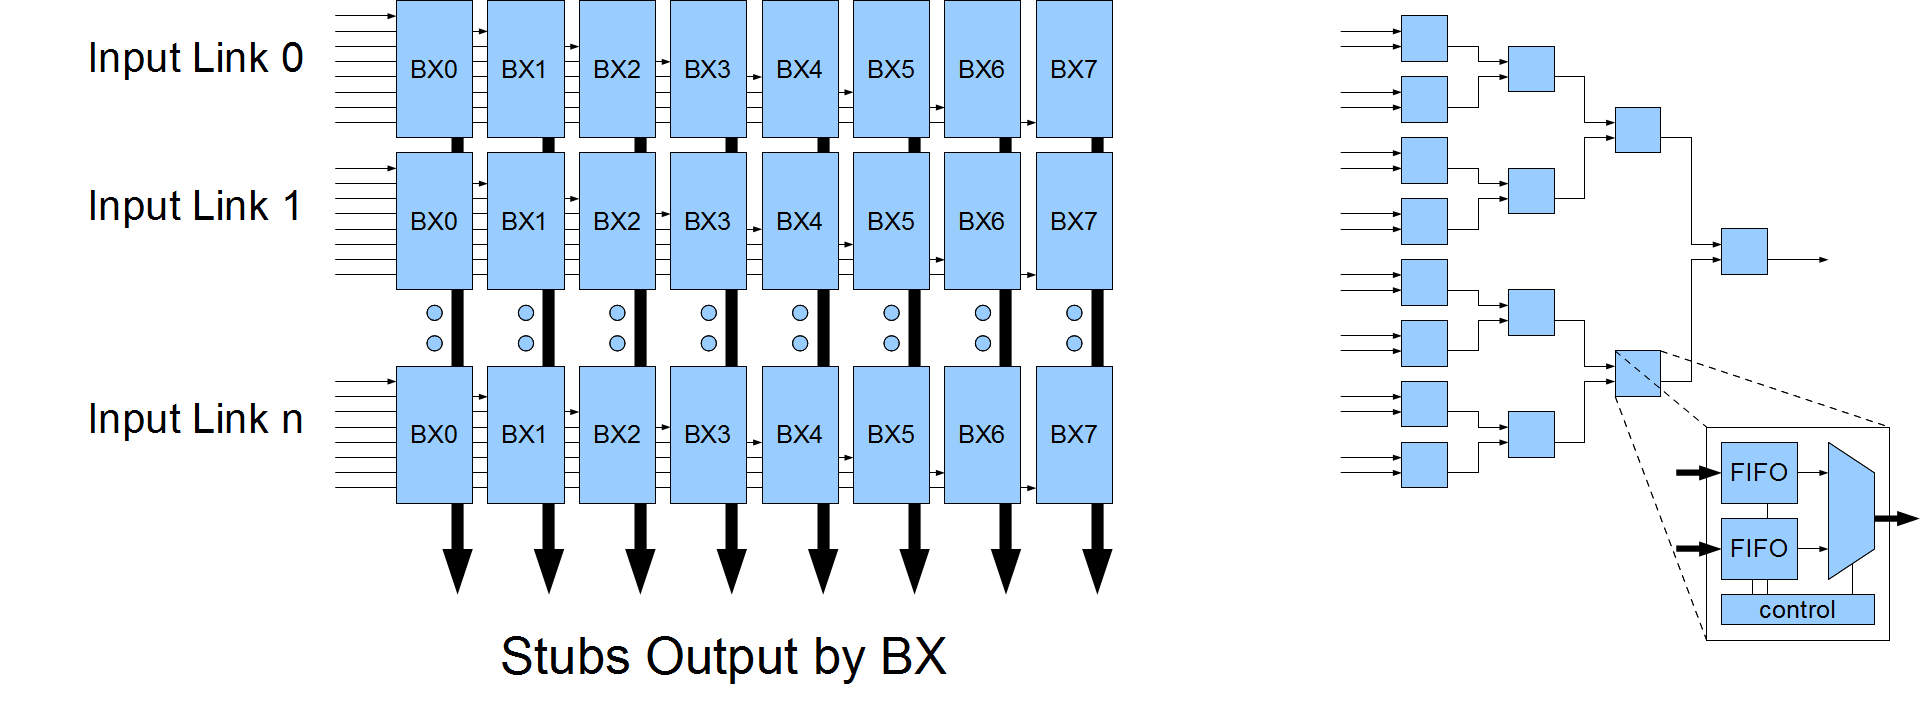
\includegraphics[width=14cm]{merge.png}
\caption{Two examples of stub merge logic. The ``parking" design (left) left uses an array of FIFOs while the ``streaming" design (right) is based around a tree of internally buffered sort nodes.}
\label{mergelogic}
\end{figure}

At this stage of the front end logic each input link has become a 32 bit wide bus synchronized to the FPGA master clock (typically 240MHz).  Each of these buses may be carrying a stub belonging to any one of 8 BX, or no stub at all.  The next step is to demultiplex stubs by BX.  For example, if the PRB FPGA has 32 RTM inputs after demultiplexing we now have 32 x 8 buses; each bus is 32 bits wide and carries stubs belonging to the same BX.

At this point we have large number of sparsely occupied buses which will need to be merged down to a few data streams prior to transmission over the full mesh backplane.  Two methods have so far been explored for performing this merge operation: parking and streaming.  

The parking style merge logic uses an 2-D array of FIFOs: rows corespond to input links and columns correspond to BX numbers, as shown in Figure{mergelogic}.  Operations on this FIFO array occur in two distinct, non-overlapping write and read phases; each phase is 200ns long in order to line up with the input train structure.  During the write phase the input buses drop stubs into the appropriate FIFOs; because the input buses are already demuliplexed the write logic is very simple and fast.  At the end of the 200ns period all input stubs have been deposited into the proper FIFOs and the readout phase can begin.  Read logic scans down the columns of the array looking for non-empty FIFOs.  When an non-empty FIFO is encountered, stubs are read out sequentially until the FIFO is empty, then the scanning process continues on down the column to the next non-empty FIFO.  The read logic is complex due to the read-ahead logic used to insure that no extra clock cycles are wasted skipping over empty FIFOs (e.g. zero suppresed readout).  At the end of the 200ns readout phase all FIFOs are reset and any remaining stubs are lost.  Write and read operations cannot occur simulaniously on the FIFO array, and thus for continuous operation the parking merge logic must be duplicated.  If we assume 32 input links then each FIFO array uses 32 x 8 = 256 FIFOs, or 512 total.  Using BlockRAM for FIFOs would then consume 17\% of the resources in the XC7VX690 FPGA.  Latency as measured from first stub in to first stub out is 200ns.

The ``stream" architecture is an alternative merge design that seeks to minimize latency through the use of binary tree elements shown in Figure {mergelogic}.  Stubs enter the merge tree and progress through tiers of nodes to the output bus.  Nodes buffer incoming stubs in small FIFOs which may be implemented in BlockRAM or distributed RAM.  Simple control logic in each node monitors the two FIFO empty flags and determines which stub will advance to the output.  Unlike the parking merge logic streaming does not have distinct write and read phases; stubs continuously flow through the tree structure to the output.  As always, care must be taken to insure that stubs from a previous event do not lurk around to corrupt the next event.  The End of Event (EOE) signal is asserted on the last clock cycle of the 200ns train and this forces all FIFOs to empty just before the next set of stubs arrives.  To implement a single 32 input merge tree 30 nodes (60 FIFOs) are required.  The complete BX Merge block requires 8 merge trees, one per BX, for a total of 240 nodes or 480 FIFOs, or about 10\% of the XC7VX690T FPGA if distributed RAM is used for the FIFOs.  Latency through the merge tree is 7 clock cycles or 29ns at 240MHz.

\subsubsection {Data Transfer Across the Full Mesh Fabric}

Stub data transfers over the full mesh backplane must always be completed in 200ns or less, as this period matches the rate which incoming trains arrive on the RTM inputs.  All Pulsar2b boards in the shelf are connected over two bidirectional lanes on the full mesh fabric; all backplane lanes are dedicated, direct, point to point connections so the overhead associated with channel sharing and bus arbitration is avoided completely.  Assuming a line rate of 10Gbps per lane then a total of about 100 stubs can be transferred from one PRB to another PRB within the 200ns window.

At any given time eight PRBs receive stub data (corresponding to the 8 BXs in the train) from other PRBs in the shelf via the backplane.  For example, as the first trains arrive at the shelf all PRBs demultiplex stubs by BX and merge them into streams which will be sent over the backplane fabric.  All PRBs send BX0 stubs to the PRB in slot 3; BX1 stubs are sent to the PRB in slot 4; BX2 stubs to slot 5; and so on for all 8 BX.  In a static configuration the mapping between destination PRB slot and BX is fixed; so in this example the PRB in slot 3 receives BX0 stubs from all other PRBs and a new event arrives every 200ns. 

\begin{table}
\centering
\caption{Example rotation scheme with ten PRBs.}
\label{rotation10table}
\begin{tabular}{|l|c|c|c|c|c|} \hline
        & T1  & T2  & T3  & T4  & T5  \\ \hline
Slot 3  & BX0 & ... & BX3 & BX2 & BX1 \\ \hline
Slot 4  & BX1 & BX0 & ... & BX3 & BX2 \\ \hline
Slot 5  & BX2 & BX1 & BX0 & ... & BX3 \\ \hline
Slot 6  & BX3 & BX2 & BX1 & BX0 & ... \\ \hline
Slot 7  & ... & BX3 & BX2 & BX1 & BX0 \\ \hline

Slot 8  & BX4 & ... & BX7 & BX6 & BX5 \\ \hline
Slot 9  & BX5 & BX4 & ... & BX7 & BX6 \\ \hline
Slot 10 & BX6 & BX5 & BX4 & ... & BX7 \\ \hline
Slot 11 & BX7 & BX6 & BX5 & BX4 & ... \\ \hline
Slot 12 & ... & BX7 & BX6 & BX5 & BX4 \\ \hline
\end{tabular}
\end{table}

In a dynamic, rotating configuration the number of possible destination PRBs is greater than eight, and the slot-BX assigments change with each new 200ns train.  There are however still only 8 destination PRBs receiving stubs from the backplane at any given time.  To illustrate this consider a shelf with ten PRBs: all ten PRBs receive stubs from RTM inputs, and all ten PRBs are eligible to receive stubs from the backplane.  Backplane transfers between PRBs still take place in 200ns, but two out of the ten PRBs receive no stubs from the backplane in a given cycle.  This rotation scheme is shown in Table \ref{rotation10table}.  Here all ten PRBs receive the first train (T1) from the RTM links.  After demulplexing and merging the stubs all PRBs send BX0 stubs over the backplane to the PRB in slot 3; all PRBs send BX1 stubs to slot 4, and so on.  The PRBs in slot 7 and 12 sit out this time and receive no stubs from the backplane.  In the next train (T2) the PRBs in slots 7 and 12 are active and receive stubs from the backplane while the PRBs in slots 3 and 8 do not.  This example rotation scheme repeats every five trains and within this 5 train cycle every PRB will receive four 200ns transfers from the backplane and rest for one 200ns period.  FIFOs in the PRB datapath (see Figure \ref{prb_fw}) act as shock absorbers and smooth out these incoming data bursts and allow for continuous data flow to the PRM mezzanine boards.  In this example the rotation scheme has increased the \emph{average} event period from 200ns to 250ns.

\subsubsection {Layer Sort Logic}

All stubs entering the PRB from the backplane fabric belong to the same BX and arrive within a 200ns window.  These stubs are then demulipexed again, this time by detector layer, and merged into six streams prior to transmission to the PRM mezzanines.  The demultiplex and merge logic is very similar to the logic described in Section \ref{merge_logic_section}.  In our baseline design we use a pair of PRMs on each PRB board; these two PRMs handle different events so we again increase our available processing by time multiplexing between the two mezzanines.  In the example rotation scheme described in the prior section the PRB receives a new event (on average) every 250ns.  Using a pair of time muliplexed PRMs doubles this period and now each PRM will see a new event every 500ns.  (This period also represents the maximum duration of PRB to PRM data transfer window, as well as the fundamental step size in the PRM pipeline stages.)

\subsection{Data Delivery Latency}
\label{section_latency}

Latency figures through the PRB are described in Table \ref{data_delivery_latency_table}.  (The observation points are marked in red on the block diagram in Figure \ref{prb_fw}.)  PRB data delivery begins at the RTM inputs (point 1) and ends at the PRM input (point 5).  For the BX and Layer merge logic the ``parking" architecture (described in Section \ref{merge_logic_section}) is assumed.  In this example eight PRBs are used and the PRB-BX mapping is static, e.g. no rotation.  Figure \ref{prb_latency_scope} shows the PRB latency as measured on hardware at the test stand.

PRM latency is described in the companion Technical Memo TM-2651-E\cite{tm2651e}.  

\begin{table}
\centering
\caption{Pattern Recognition Board Latency.}
\label{data_delivery_latency_table}
\begin{tabular}{|l|l|c|c|c|} \hline
Observation Point & Description                       & Latency(ns) & Start(ns)  & End(ns) \\ \hline
1                 & Module data arrives at RTM inputs &             & 0          & 200     \\ \hline
                  & MGT RX and alignment              & 130         &            &         \\ \hline
                  & Unpack PRBF and format            & 200         &            &         \\ \hline
2                 & Stubs after formatting            &             & 330        & 530     \\ \hline
                  & Stub BX demux and merge (park)    & 200         &            &         \\ \hline
                  & MGT TX                            & 100         &            &         \\ \hline
3                 & Stub transfer on full mesh        &             & 630        & 830     \\ \hline
                  & MGT RX and alignment              & 130         &            &         \\ \hline
                  & Stub Layer demux and merge (park) & 200         &            &         \\ \hline
4                 & Stubs after layer merge           &             & 960        & 1160    \\ \hline
                  & PRM demux and FIFO                & 25          &            &         \\ \hline
                  & MGT TX                            & 100         &            &         \\ \hline
5                 & Stub transfer to PRM              &             & 1085       & 1585    \\ \hline
\end{tabular}
\end{table}

\begin{figure}
\centering
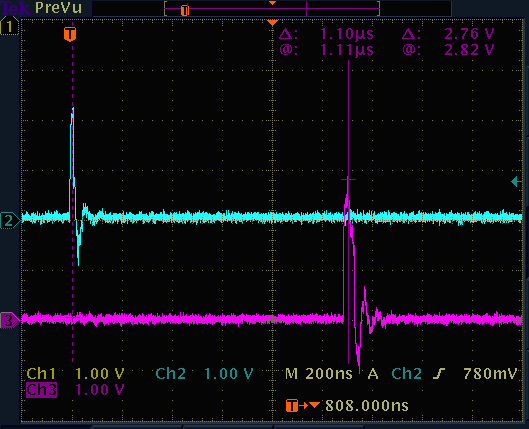
\includegraphics[width=12cm]{prb_latency_scope.png}
\caption{PRB latency as measured on the test stand hardware.  Channel 2 (blue) shows the arrival of the first stub into the PRB from the RTM (aka point 1)  Channel 3 (purple) shows the first stub arriving at the PRM input (point 5).  The time between this markers is shown as 1100ns which is in good agreement with our PRB latency estimate of 1085ns from Table \ref{data_delivery_latency_table}. }
\label{prb_latency_scope}
\end{figure}

\clearpage
\newpage
\appendices

\section{Full Mesh and Direct Flow Architecture}
\label{Appendix_DirectFlow}

\begin{figure}
\centering
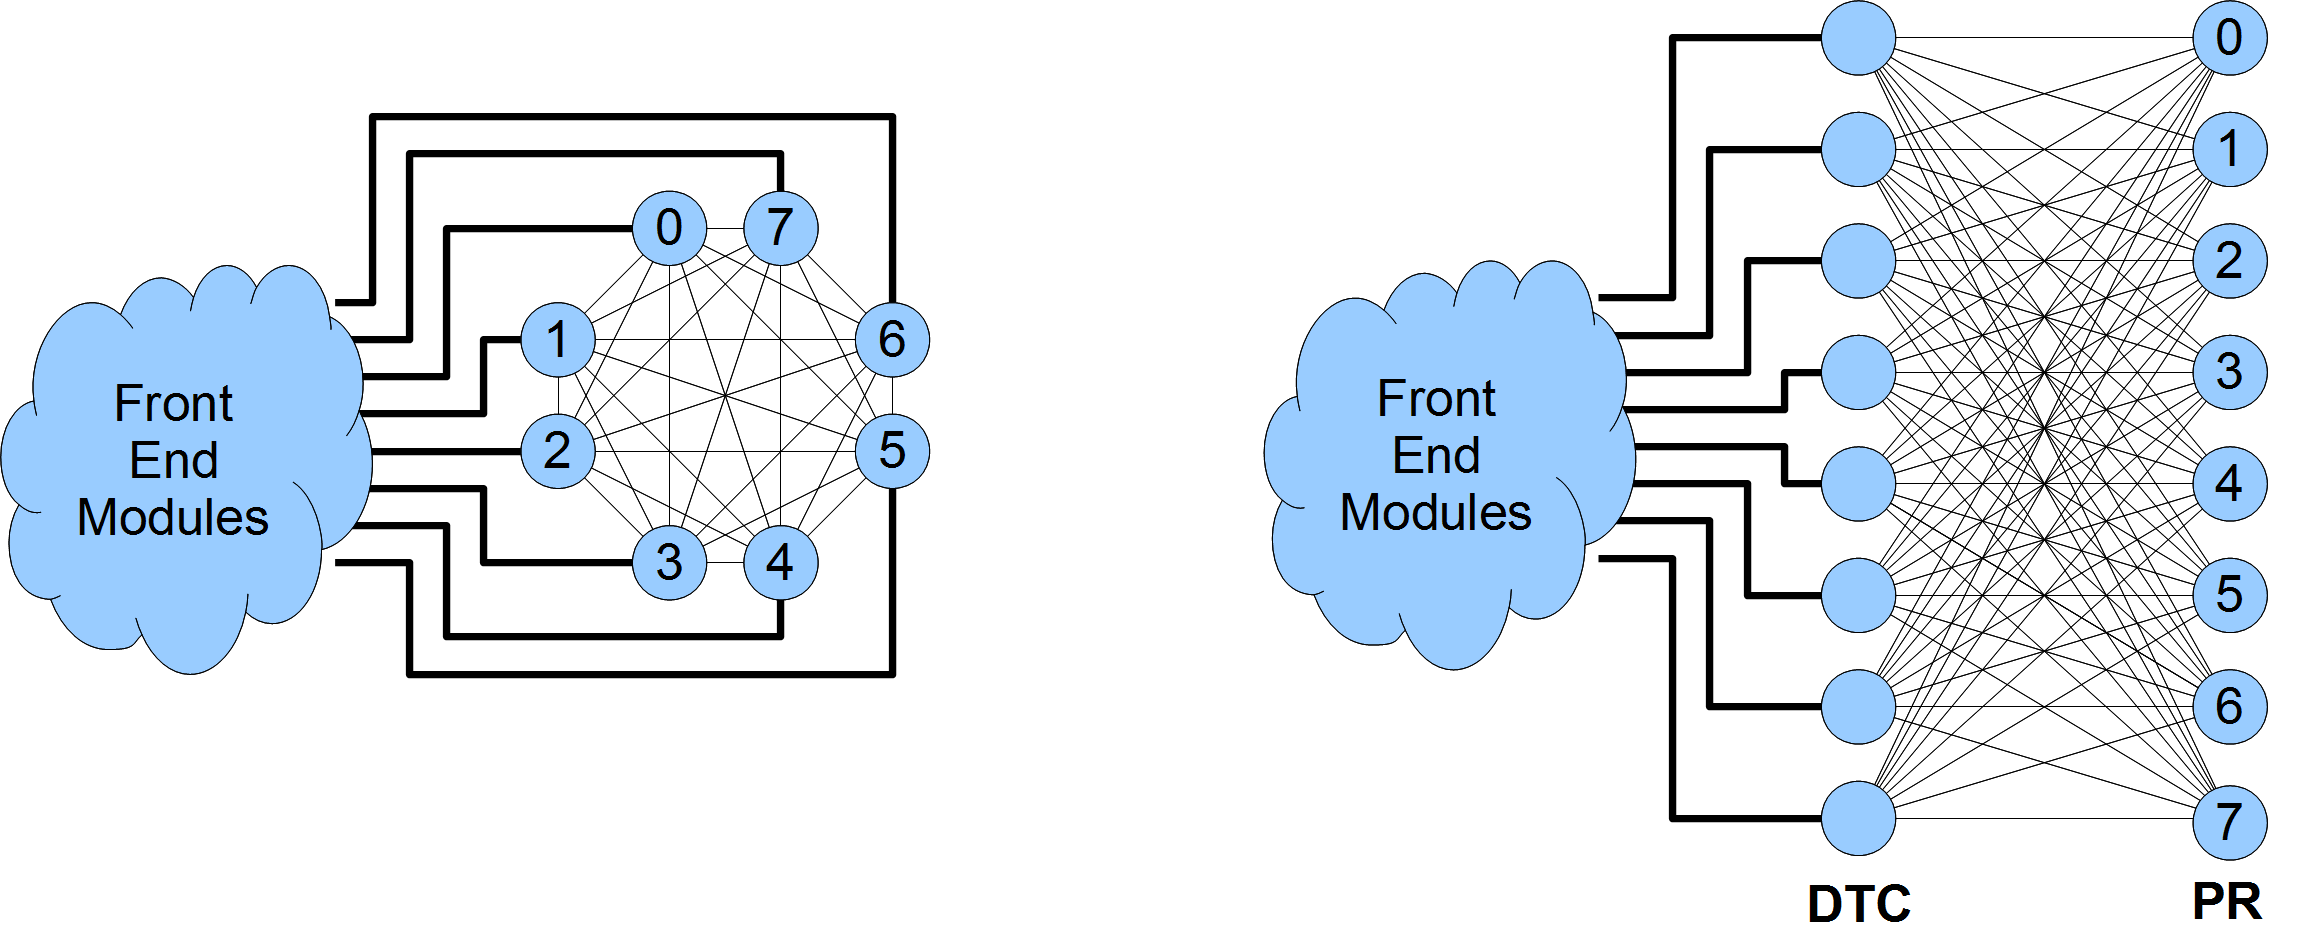
\includegraphics[width=14cm]{arch.png}
\caption{Two simple examples of data distribution architectures based on a full mesh network (left) and ``direct flow" fibers (right).}
\label{fig_arch_compare}
\end{figure}

Several groups have proposed designs for the CMS L1 Tracking Trigger hardware.  While all tracking trigger hardware designs make use of time multiplexing techniques, the data data delivery mechanism differs substantially in terms of how individual boards are connected together.  Two network topologies have emerged: full mesh and direct flow; in this section we will discuss the merits of each system.

\subsection{Full Mesh}

Our data delivery scheme is based around the full mesh network; having abundant non-blocking high speed communication channels \emph{between all boards in the shelf} is essential to our data delivery scheme and central to how our time multiplexed transfer scheme works (see Section \ref{section_prb} for details).  An example system based around all full mesh network is shown on the left side of Figure \ref{fig_arch_compare}.  Here all eight boards receive fixed length ``trains" from the front end modules.  Within each fixed length train there are varying numbers of stubs for up to eight bunch crossings (BX).  Upon reception of these trains the boards demultiplex and combine incoming stubs by BX and these data streams are output to the full mesh network. In this simple example there are eight boards so the BX to board assignments are static: the full mesh network assures that each board sends all stubs belonging to BX0 to board 0; all stubs belonging to BX1 are routed to board 1, etc.  Likewise, board 0 receives all stubs belonging to BX0 from all boards; board 1 receives all BX1 stubs, etc.  Now all stubs for a given BX are in one place pattern recognition and track finding can begin.

\subsection{Direct Flow}

The system shown on the right in Figure \ref{fig_arch_compare} is an example of the so called ``direct flow" architecture.  
The most significant difference between full mesh and direct flow is that with the latter case the demultipexing and processing functions take place in separate boards.  Front end modules connect to DTC boards, which form the first hardware layer where stub demultiplexing takes place.  The DTC boards send stubs to the second hardware layer where PR boards process the event.  The fiber network between the DTC boards and PR boards in some ways functions like a full mesh network, and thus delivers all stubs belonging to one event into a given PR board.  Consequently no communication between PR boards is required.

\subsubsection{DTC Boards}

The purpose of the DTC board is to receive stubs from the front end modules, demultiplex the stubs by BX and merge these streams into output links which go to the PR boards.  Thus the number of DTC output links equals the time muliplex period.  In our simple example each DTC board has 8 outputs and sends to eight PR boards.

In a direct flow system challenges arise when a DTC board needs to send to more than one geometric region, for example when stubs need to shared across tower or sector boundaries.  Since sharing between PR boards takes cannot occur it is solely the responsibility of the DTC to duplicate stub data and drive the extra output links to PR boards in other regions.  When additional DTC outputs are required they must be added in groups, one link per TM period.  As we will see in subsequent sections the region boundaries have been carefully selected as to minimize the number of regions and number of DTC outputs required.

\subsubsection{Link Bandwidth}

It is generally understood that in the direct flow scheme there is one and only one fiber link connecting a DTC - PR board pair.









is hardware layer called the DTC, and the pattern recogition and other processing occurs in the PR boards.  DTC boards and PR boards are connected with simplex fiber optic links.  Since demultiplexing is done in the DTC there is no need for communication between PR boards; this simplifies somewhat the design of the PR board I/O, however, as we will see the fiber network between the DTC and PR boards can grow quite complex.


The fixed length trains generated by the front end modules are received by the DTC boards.  The DTC boards demultiplex stubs by BX and send these stubs to the appropriate PR boards over fibers.  

The number of PR boards determines the time multiplex period in the direct flow architecture.  The number of PR boards determines the number of outputs per DTC board as well.  




\subsubsection{Fiber Mapping}
bundles of 12 fibers
mixer boxes



















\newpage
\section{MGT Channel Assignments}
\label{Appendix_MGTs}

Some TX or RX differential pairs have been flipped to improve the physical PCB layout.  These flipped pairs are indicated by a Y in the TX-INV or RX-INV columns.

% apply resizebox to make this large table fit on a single page 

\begin{table}[htp]
\centering
\caption{Pulsar2b FPGA MGT Channel Assignments, Left Column.}
\begin{tabular}{|l|l|l|l|l|l|} \hline
L-Channel & Type & Quad & Location & TX-INV & RX-INV \\ \hline
FMC1-0 & FMC & 219-3 & MGT-X0Y39 & Y & Y \\ \hline
FMC1-1 & FMC & 219-2 & MGT-X0Y38 & . & Y \\ \hline
FMC1-2 & FMC & 219-1 & MGT-X0Y37 & . & Y \\ \hline
FMC2-0 & FMC & 219-0 & MGT-X0Y36 & . & . \\ \hline
FMC2-1 & FMC & 218-3 & MGT-X0Y35 & Y & . \\ \hline
FMC2-2 & FMC & 218-2 & MGT-X0Y34 & . & . \\ \hline
Q0-1 & RTM & 218-1 & MGT-X0Y33 & . & . \\ \hline
Q0-2 & RTM & 218-0 & MGT-X0Y32 & . & . \\ \hline
Q0-3 & RTM & 217-3 & MGT-X0Y31 & . & . \\ \hline
Q0-4 & RTM & 217-2 & MGT-X0Y30 & . & . \\ \hline
Q1-1 & RTM & 217-1 & MGT-X0Y29 & . & . \\ \hline
Q1-2 & RTM & 217-0 & MGT-X0Y28 & . & . \\ \hline
Q1-3 & RTM & 216-3 & MGT-X0Y27 & . & . \\ \hline
Q1-4 & RTM & 216-2 & MGT-X0Y26 & . & . \\ \hline
Q2-1 & RTM & 216-1 & MGT-X0Y25 & . & . \\ \hline
Q2-2 & RTM & 216-0 & MGT-X0Y24 & . & . \\ \hline
Q2-3 & RTM & 215-3 & MGT-X0Y23 & . & . \\ \hline
Q2-4 & RTM & 215-2 & MGT-X0Y22 & . & . \\ \hline
Q3-1 & RTM & 215-1 & MGT-X0Y21 & . & . \\ \hline
Q3-2 & RTM & 215-0 & MGT-X0Y20 & . & . \\ \hline \hline
Q3-3 & RTM & 214-3 & MGT-X0Y19 & . & . \\ \hline
Q3-4 & RTM & 214-2 & MGT-X0Y18 & . & . \\ \hline
Q4-1 & RTM & 214-1 & MGT-X0Y17 & . & . \\ \hline
Q4-2 & RTM & 214-0 & MGT-X0Y16 & . & Y \\ \hline
Q4-3 & RTM & 213-3 & MGT-X0Y15 & . & . \\ \hline
Q4-4 & RTM & 213-2 & MGT-X0Y14 & . & . \\ \hline
Q5-1 & RTM & 213-1 & MGT-X0Y13 & . & . \\ \hline
Q5-2 & RTM & 213-0 & MGT-X0Y12 & . & . \\ \hline
Q5-3 & RTM & 212-3 & MGT-X0Y11 & Y & . \\ \hline
Q5-4 & RTM & 212-2 & MGT-X0Y10 & . & Y \\ \hline
Q6-1 & RTM & 212-1 & MGT-X0Y9 & . & .  \\ \hline
Q6-2 & RTM & 212-0 & MGT-X0Y8 & . & .  \\ \hline
Q6-3 & RTM & 211-3 & MGT-X0Y7 & . & .  \\ \hline
Q6-4 & RTM & 211-2 & MGT-X0Y6 & Y & .  \\ \hline
Q7-1 & RTM & 211-1 & MGT-X0Y5 & . & .  \\ \hline
Q7-2 & RTM & 211-0 & MGT-X0Y4 & . & .  \\ \hline
Q7-3 & RTM & 210-3 & MGT-X0Y3 & . & .  \\ \hline
Q7-4 & RTM & 210-2 & MGT-X0Y2 & . & .  \\ \hline
Q8-1 & RTM & 210-1 & MGT-X0Y1 & . & .  \\ \hline
Q8-2 & RTM & 210-0 & MGT-X0Y0 & . & .  \\ \hline
\end{tabular}
\end{table}

\newpage

\begin{table}[htp]
\centering
\caption{Pulsar2b FPGA MGT Channel Assignments, Right Column.}
\begin{tabular}{|l|l|l|l|l|l|} \hline
R-Channel & Type & Quad & Location & TX-INV & RX-INV \\ \hline
FMC4-2 & FMC & 119-3 & MGT-X1Y39 & . & Y\\ \hline
FMC4-1 & FMC & 119-2 & MGT-X1Y38 & Y & .\\ \hline
FMC4-0 & FMC & 119-1 & MGT-X1Y37 & Y & Y\\ \hline
FMC3-2 & FMC & 119-0 & MGT-X1Y36 & . & .\\ \hline
FMC3-1 & FMC & 118-3 & MGT-X1Y35 & . & .\\ \hline
FMC3-0 & FMC & 118-2 & MGT-X1Y34 & . & Y\\ \hline
C1P0 & Fabric & 118-1 & MGT-X1Y33 & . & .\\ \hline
C1P1 & Fabric & 118-0 & MGT-X1Y32 & . & .\\ \hline
C1P2 & Fabric & 117-3 & MGT-X1Y31 & . & .\\ \hline
C1P3 & Fabric & 117-2 & MGT-X1Y30 & . & .\\ \hline
C2P0 & Fabric & 117-1 & MGT-X1Y29 & . & .\\ \hline
C2P1 & Fabric & 117-0 & MGT-X1Y28 & . & .\\ \hline
C3P0 & Fabric & 116-3 & MGT-X1Y27 & . & .\\ \hline
C3P1 & Fabric & 116-2 & MGT-X1Y26 & . & .\\ \hline
C4P0 & Fabric & 116-1 & MGT-X1Y25 & . & .\\ \hline
C4P1 & Fabric & 116-0 & MGT-X1Y24 & . & .\\ \hline
C5P0 & Fabric & 115-3 & MGT-X1Y23 & . & .\\ \hline
C5P1 & Fabric & 115-2 & MGT-X1Y22 & . & .\\ \hline
C6P0 & Fabric & 115-1 & MGT-X1Y21 & . & .\\ \hline
C6P1 & Fabric & 115-0 & MGT-X1Y20 & . & .\\ \hline \hline
C7P0 & Fabric & 114-3 & MGT-X1Y19 & . & Y\\ \hline
C7P1 & Fabric & 114-2 & MGT-X1Y18 & . & .\\ \hline
C8P0 & Fabric & 114-1 & MGT-X1Y17 & . & .\\ \hline
C8P1 & Fabric & 114-0 & MGT-X1Y16 & . & .\\ \hline
C9P0 & Fabric & 113-3 & MGT-X1Y15 & . & .\\ \hline
C9P1 & Fabric & 113-2 & MGT-X1Y14 & . & .\\ \hline
C10P0 & Fabric & 113-1 & MGT-X1Y13 & . & .\\ \hline
C10P1 & Fabric & 113-0 & MGT-X1Y12 & . & .\\ \hline
C11P0 & Fabric & 112-3 & MGT-X1Y11 & . & .\\ \hline
C11P1 & Fabric & 112-2 & MGT-X1Y10 & . & .\\ \hline
C12P0 & Fabric & 112-1 & MGT-X1Y9 & . & .\\ \hline
C12P1 & Fabric & 112-0 & MGT-X1Y8 & . & .\\ \hline
C13P0 & Fabric & 111-3 & MGT-X1Y7 & . & .\\ \hline
C13P1 & Fabric & 111-2 & MGT-X1Y6 & Y & .\\ \hline
Q9-4 & RTM & 111-1 & MGT-X1Y5 & . & .\\ \hline
Q9-3 & RTM & 111-0 & MGT-X1Y4 & Y & .\\ \hline
Q9-2 & RTM & 110-3 & MGT-X1Y3 & Y & Y\\ \hline
Q9-1 & RTM & 110-2 & MGT-X1Y2 & Y & Y\\ \hline
Q8-4 & RTM & 110-1 & MGT-X1Y1 & Y & Y\\ \hline
Q8-3 & RTM & 110-0 & MGT-X1Y0 & Y & Y\\ \hline
\end{tabular}
\end{table}

\newpage
\section{LVDS Signal Assignments for Mezzanines}
\label{Appendix_LVDS}

The parallel LVDS interface consists of two clock pairs and 34 data pairs per FMC connector.  The clock pairs CLK0 and CLK1 are generally understood to be OUTPUTS FROM the mezzanine card TO the Pulsar2b FPGA.  If a clock needs to be sent from the Pulsar2b FPGA to the mezzanine card use the LA00 pair for this purpose.  The PSNT pin is grounded on the FMC mezzanine card.  On the Pulsar2b FPGA this pin should be an input with an internal weak pullup resistor enabled.  Thus this signal acts as an active low signal to indicate that an FMC mezzanine is installed.  LVDS P/N pairs marked with * have been flipped to make the layout cleaner and should be inverted in firmware.

\begin{table}[htp]
\centering
\caption{Pulsar2b LVDS Signal Assignments for Mezzanines 1 and 2.}
\begin{tabular}{|l|l|l|l||l|l|l|l|} \hline
Pin & Name & Pin & Name & Pin & Name & Pin & Name \\ \hline \hline
H29 & FB1\_CLK0\_N & E32 & FB1\_LA16\_N* & H32 & FB2\_CLK0\_N* & T24 & FB2\_LA16*\_N\\ \hline
H28 & FB1\_CLK0\_P & E33 & FB1\_LA16\_P* & H33 & FB2\_CLK0\_P* & T25 & FB2\_LA16*\_P\\ \hline
J27 & FB1\_CLK1\_N & K28 & FB1\_LA17\_N* & H30 & FB2\_CLK1\_N* & U25 & FB2\_LA17*\_N\\ \hline
K27 & FB1\_CLK1\_P & J29 & FB1\_LA17\_P* & G30 & FB2\_CLK1\_P* & U26 & FB2\_LA17*\_P\\ \hline
G33 & FB1\_LA00\_N* & A30 & FB1\_LA18\_N* & G28 & FB2\_LA00\_N* & A24 & FB2\_LA18*\_N\\ \hline
F33 & FB1\_LA00\_P* & A31 & FB1\_LA18\_P* & F28 & FB2\_LA00\_P* & A25 & FB2\_LA18*\_P\\ \hline
G31 & FB1\_LA01\_N* & M28 & FB1\_LA19\_N* & D24 & FB2\_LA01\_N* & B27 & FB2\_LA19\_N\\ \hline
G32 & FB1\_LA01\_P* & L29 & FB1\_LA19\_P* & D25 & FB2\_LA01\_P* & C27 & FB2\_LA19\_P\\ \hline
F30 & FB1\_LA02\_N* & C32 & FB1\_LA20\_N* & R27 & FB2\_LA02\_N* & C28 & FB2\_LA20*\_N\\ \hline
F31 & FB1\_LA02\_P* & C33 & FB1\_LA20\_P* & P27 & FB2\_LA02\_P* & B28 & FB2\_LA20*\_P\\ \hline
M33 & FB1\_LA03\_N & D30 & FB1\_LA21\_N* & E23 & FB2\_LA03\_N* & B25 & FB2\_LA21\_N\\ \hline
N33 & FB1\_LA03\_P & D31 & FB1\_LA21\_P* & E24 & FB2\_LA03\_P* & C25 & FB2\_LA21\_P\\ \hline
L33 & FB1\_LA04\_N* & E31 & FB1\_LA22\_N* & G23 & FB2\_LA04\_N* & F26 & FB2\_LA22*\_N\\ \hline
K33 & FB1\_LA04\_P* & D32 & FB1\_LA22\_P* & F23 & FB2\_LA04\_P* & E26 & FB2\_LA22*\_P\\ \hline
D29 & FB1\_LA05\_N* & H27 & FB1\_LA23\_N* & H23 & FB2\_LA05\_N* & D26 & FB2\_LA23*\_N\\ \hline
C29 & FB1\_LA05\_P* & G27 & FB1\_LA23\_P* & H24 & FB2\_LA05\_P* & D27 & FB2\_LA23*\_P\\ \hline
A33 & FB1\_LA06\_N & T28 & FB1\_LA24\_N* & G25 & FB2\_LA06\_N* & T26 & FB2\_LA24*\_N\\ \hline
B33 & FB1\_LA06\_P & T29 & FB1\_LA24\_P* & G26 & FB2\_LA06\_P* & R26 & FB2\_LA24*\_P\\ \hline
K32 & FB1\_LA07\_N* & U30 & FB1\_LA25\_N* & K23 & FB2\_LA07\_N* & C23 & FB2\_LA25*\_N\\ \hline
J32 & FB1\_LA07\_P* & T30 & FB1\_LA25\_P* & K24 & FB2\_LA07\_P* & C24 & FB2\_LA25*\_P\\ \hline
E27 & FB1\_LA08\_N* & B30 & FB1\_LA26\_N & F24 & FB2\_LA08\_N* & P25 & FB2\_LA26*\_N\\ \hline
E28 & FB1\_LA08\_P* & C30 & FB1\_LA26\_P & F25 & FB2\_LA08\_P* & P26 & FB2\_LA26*\_P\\ \hline
R33 & FB1\_LA09\_N & A28 & FB1\_LA27\_N* & U27 & FB2\_LA09\_N* & A23 & FB2\_LA27\_N\\ \hline
T33 & FB1\_LA09\_P & A29 & FB1\_LA27\_P* & U28 & FB2\_LA09\_P* & B23 & FB2\_LA27\_P\\ \hline
J30 & FB1\_LA10\_N* & P32 & FB1\_LA28\_N & A26 & FB2\_LA10\_N & R28 & FB2\_LA28*\_N\\ \hline
J31 & FB1\_LA10\_P* & R32 & FB1\_LA28\_P & B26 & FB2\_LA10\_P & R29 & FB2\_LA28*\_P\\ \hline
M31 & FB1\_LA11\_N* & U32 & FB1\_LA29\_N* & J25 & FB2\_LA11\_N* & N28 & FB2\_LA29*\_N\\ \hline
M32 & FB1\_LA11\_P* & U33 & FB1\_LA29\_P* & J26 & FB2\_LA11\_P* & N29 & FB2\_LA29*\_P\\ \hline
E29 & FB1\_LA12\_N & T31 & FB1\_LA30\_N* & M23 & FB2\_LA12\_N* & L24 & FB2\_LA30*\_N\\ \hline
F29 & FB1\_LA12\_P & R31 & FB1\_LA30\_P* & L23 & FB2\_LA12\_P* & L25 & FB2\_LA30*\_P\\ \hline
L31 & FB1\_LA13\_N* & P31 & FB1\_LA31\_N* & J24 & FB2\_LA13\_N* & L26 & FB2\_LA31*\_N\\ \hline
K31 & FB1\_LA13\_P* & N32 & FB1\_LA31\_P* & H25 & FB2\_LA13\_P* & K26 & FB2\_LA31*\_P\\ \hline
B31 & FB1\_LA14\_N* & L28 & FB1\_LA32\_N* & N23 & FB2\_LA14\_N* & U23 & FB2\_LA32*\_N\\ \hline
B32 & FB1\_LA14\_P* & K29 & FB1\_LA32\_P* & N24 & FB2\_LA14\_P* & T23 & FB2\_LA32*\_P\\ \hline
N30 & FB1\_LA15\_N* & P29 & FB1\_LA33\_N* & R23 & FB2\_LA15\_N* & N25 & FB2\_LA33*\_N\\ \hline
M30 & FB1\_LA15\_P* & P30 & FB1\_LA33\_P* & R24 & FB2\_LA15\_P* & M25 & FB2\_LA33*\_P\\ \hline
    &            & U31 & FB1\_PSNT\_L &     &            & L30 & FB2\_PSNT\_L\\ \hline
\end{tabular}
\end{table}

\newpage

\begin{table}[htp]
\centering
\caption{Pulsar2b LVDS Signal Assignments for Mezzanines 3 and 4.}
\begin{tabular}{|l|l|l|l||l|l|l|l|} \hline
Pin & Name & Pin & Name & Pin & Name & Pin & Name \\ \hline \hline
H14 & FB3\_CLK0\_N & M22 & FB3\_LA16\_N & G17 & FB4\_CLK0\_N & H12 & FB4\_LA16\_N* \\ \hline
H15 & FB3\_CLK0\_P & N22 & FB3\_LA16\_P & H18 & FB4\_CLK0\_P & G12 & FB4\_LA16\_P* \\ \hline
J14 & FB3\_CLK1\_N & J20 & FB3\_LA17\_N & J16 & FB4\_CLK1\_N & J17 & FB4\_LA17\_N* \\ \hline
J15 & FB3\_CLK1\_P & J21 & FB3\_LA17\_P & K17 & FB4\_CLK1\_P & H17 & FB4\_LA17\_P* \\ \hline
G22 & FB3\_LA00\_N & B16 & FB3\_LA18\_N* & C18 & FB4\_LA00\_N* & M16 & FB4\_LA18\_N \\ \hline
H22 & FB3\_LA00\_P & A16 & FB3\_LA18\_P* & B18 & FB4\_LA00\_P* & M17 & FB4\_LA18\_P \\ \hline
C22 & FB3\_LA01\_N* & L19 & FB3\_LA19\_N* & D16 & FB4\_LA01\_N & R18 & FB4\_LA19\_N* \\ \hline
B22 & FB3\_LA01\_P* & K19 & FB3\_LA19\_P* & D17 & FB4\_LA01\_P & R17 & FB4\_LA19\_P* \\ \hline
E21 & FB3\_LA02\_N & M20 & FB3\_LA20\_N* & B17 & FB4\_LA02\_N & L16 & FB4\_LA20\_N* \\ \hline
E22 & FB3\_LA02\_P & L20 & FB3\_LA20\_P* & C17 & FB4\_LA02\_P & K16 & FB4\_LA20\_P* \\ \hline
D21 & FB3\_LA03\_N & P20 & FB3\_LA21\_N & D14 & FB4\_LA03\_N & K12 & FB4\_LA21\_N* \\ \hline
D22 & FB3\_LA03\_P & P21 & FB3\_LA21\_P & D15 & FB4\_LA03\_P & J12 & FB4\_LA21\_P* \\ \hline
C20 & FB3\_LA04\_N & K21 & FB3\_LA22\_N & C14 & FB4\_LA04\_N & M13 & FB4\_LA22\_N* \\ \hline
D20 & FB3\_LA04\_P & L21 & FB3\_LA22\_P & C15 & FB4\_LA04\_P & L13 & FB4\_LA22\_P* \\ \hline
C19 & FB3\_LA05\_N & U21 & FB3\_LA23\_N & E13 & FB4\_LA05\_N & K13 & FB4\_LA23\_N \\ \hline
D19 & FB3\_LA05\_P & U22 & FB3\_LA23\_P & E14 & FB4\_LA05\_P & K14 & FB4\_LA23\_P \\ \hline
B21 & FB3\_LA06\_N* & L18 & FB3\_LA24\_N & B15 & FB4\_LA06\_N* & N13 & FB4\_LA24\_N \\ \hline
A21 & FB3\_LA06\_P* & M18 & FB3\_LA24\_P & A15 & FB4\_LA06\_P* & N14 & FB4\_LA24\_P \\ \hline
J22 & FB3\_LA07\_N & G18 & FB3\_LA25\_N* & E12 & FB4\_LA07\_N* & L14 & FB4\_LA25\_N \\ \hline
K22 & FB3\_LA07\_P & F18 & FB3\_LA25\_P* & D12 & FB4\_LA07\_P* & M15 & FB4\_LA25\_P \\ \hline
E18 & FB3\_LA08\_N & T20 & FB3\_LA26\_N & C12 & FB4\_LA08\_N & R16 & FB4\_LA26\_N* \\ \hline
E19 & FB3\_LA08\_P & U20 & FB3\_LA26\_P & C13 & FB4\_LA08\_P & P16 & FB4\_LA26\_P* \\ \hline
G20 & FB3\_LA09\_N & N19 & FB3\_LA27\_N & G16 & FB4\_LA09\_N* & T15 & FB4\_LA27\_N \\ \hline
H20 & FB3\_LA09\_P & N20 & FB3\_LA27\_P & F16 & FB4\_LA09\_P* & T16 & FB4\_LA27\_P \\ \hline
B20 & FB3\_LA10\_N* & R19 & FB3\_LA28\_N & A13 & FB4\_LA10\_N & R12 & FB4\_LA28\_N* \\ \hline
A20 & FB3\_LA10\_P* & T19 & FB3\_LA28\_P & A14 & FB4\_LA10\_P & P12 & FB4\_LA28\_P* \\ \hline
F19 & FB3\_LA11\_N & R21 & FB3\_LA29\_N* & F13 & FB4\_LA11\_N & M12 & FB4\_LA29\_N \\ \hline
F20 & FB3\_LA11\_P & T21 & FB3\_LA29\_P* & F14 & FB4\_LA11\_P & N12 & FB4\_LA29\_P \\ \hline
G21 & FB3\_LA12\_N* & U16 & FB3\_LA30\_N & G15 & FB4\_LA12\_N* & P15 & FB4\_LA30\_N* \\ \hline
F21 & FB3\_LA12\_P* & U17 & FB3\_LA30\_P & F15 & FB4\_LA12\_P* & N15 & FB4\_LA30\_P* \\ \hline
J19 & FB3\_LA13\_N* & T18 & FB3\_LA31\_N & H13 & FB4\_LA13\_N* & V15 & FB4\_LA31\_N* \\ \hline
H19 & FB3\_LA13\_P* & U18 & FB3\_LA31\_P & G13 & FB4\_LA13\_P* & U15 & FB4\_LA31\_P* \\ \hline
A18 & FB3\_LA14\_N & E16 & FB3\_LA32\_N & B12 & FB4\_LA14\_N & U13 & FB4\_LA32\_N* \\ \hline
A19 & FB3\_LA14\_P & E17 & FB3\_LA32\_P & B13 & FB4\_LA14\_P & T13 & FB4\_LA32\_P* \\ \hline
R22 & FB3\_LA15\_N* & N17 & FB3\_LA33\_N & R13 & FB4\_LA15\_N & R14 & FB4\_LA33\_N* \\ \hline
P22 & FB3\_LA15\_P* & P17 & FB3\_LA33\_P & T14 & FB4\_LA15\_P & P14 & FB4\_LA33\_P* \\ \hline
    &            & M21 & FB3\_PSNT\_L &     &            & N18 & FB4\_PSNT\_L \\ \hline
\end{tabular}
\end{table}

\newpage
\section{Pulsar2b Board Sensors}
\label{Appendix_Sensors}

Some voltage regulators are not powered up until the board is in the M4 active state.  Attempting to read an unpowered sensor will return garbage.  The Fermilab IPMC software automatically zeros out all unpowered sensor readings.

\begin{table}[htp]
\centering
\caption{Pulsar2b Board Sensors.}
\begin{tabular}{|l|l|l|l|l|l|l|} \hline
Device & Ref & I2C Address& Parameter & Type & Units & Read \\ \hline
\hline
EBDW025A0B41Z & U9& 011 0011 & Temperature & float & C & anytime \\ \cline{4-7}
12V bus converter&&&Vin&float&V&anytime \\ \cline{4-7}
&&&Vout&float&V&anytime \\ \cline{4-7}
&&&Iout&float&A&anytime \\ \hline
\hline
UDT020A0X3-SRZ&U23&010 0000&OverTemp&boolean&&M4 \\ \cline{4-7}
voltage regulator&&&Vin&float&V&M4 \\ \cline{4-7}
MGTAVTT&&&Vout&float&V&M4 \\ \cline{4-7}
&&&Iout&float&A&M4 \\ \hline
\hline
UDT020A0X3-SRZ&U16&011 0000&OverTemp&boolean&&M4 \\ \cline{4-7}
voltage regulator&&&Vin&float&V&M4 \\ \cline{4-7}
VCC3V3&&&Vout&float&V&M4 \\ \cline{4-7}
&&&Iout&float&A&M4 \\ \hline
\hline
MDT040A0X3-SRPHZ&U17&010 0010&OverTemp&boolean&&M4 \\ \cline{4-7}
voltage regulator&&&Vin&float&V&M4 \\ \cline{4-7}
VCC1V0&&&Vout&float&V&M4 \\ \cline{4-7}
&&&Iout&float&A&M4 \\ \hline
\hline
PDT006A0X3-SRZ&U18&011 0010&OverTemp&boolean&&M4 \\ \cline{4-7}
voltage regulator&&&Vin&float&V&M4 \\ \cline{4-7}
VCC1V8&&&Vout&float&V&M4 \\ \cline{4-7}
&&&Iout&float&A&M4 \\ \hline
\hline
MDT040A0X3-SRPHZ&U21&010 0011&OverTemp&boolean&&M4 \\ \cline{4-7}
voltage regulator&&&Vin&float&V&M4 \\ \cline{4-7}
MGTAVCC&&&Vout&float&V&M4 \\ \cline{4-7}
&&&Iout&float&A&M4 \\ \hline
\hline
TPS2459&U20&000 1000&MP Good&boolean&&anytime \\ \cline{4-7}
RTM power controller&&&MP Fault&boolean&&anytime \\ \cline{4-7}
&&&PWR Good&boolean&&anytime \\ \cline{4-7}
&&&PWR Fault&boolean&&anytime \\ \hline
\hline
PIM400KZ&U8&010 1111&Temperature&float&C&anytime \\ \cline{4-7}
Power Input Module&&&Vholdup&float&V&anytime \\ \cline{4-7}
&&&Iout&float&A&anytime \\ \cline{4-7}
&&&Vin\_a&float&V&anytime \\ \cline{4-7}
&&&Vin\_b&float&V&anytime \\ \hline
\hline
LTC2990&U2&100 1100&Ambient air temp&float&C&anytime \\ \cline{4-7}
Temperature Sensor&&(sensor bus)&FPGA die temp&float&C&anytime \\ \cline{4-7}
&&&3.3V management voltage&float&V&anytime \\ \hline
\end{tabular}
\end{table}



\newpage
\begin{thebibliography}{77}
\small

\bibitem{fnal} Fermi National Accelerator Laboratory\\
Batavia, Illinois 60510 USA\\
http://www.fnal.gov

\bibitem{cern} CERN\\
https://www.cern.ch

% \bibitem{dataformatter} Dataformatter FTK JINST 2013 paper or FNAL tech memo here

\bibitem{pulsar2a} Dataformatter IEEE RT 2013 conf record

\bibitem{picmg30} PICMG 3.0 R3 Spec

\bibitem{picmg38} PICMG 3.8 Intelligent RTM Zone-3A Spec

\bibitem{qsfp} QSFP+ Transceiver Specification SFF-86XX  EIA-964/SFF-8436

\bibitem{cern_ipmc} CERN IPMC design

\bibitem{lapp_ipmc} LAPP IPMC design

\bibitem{wisc_ipmc} UW Madison IPMC design

\bibitem{tm2651e} Fermilab Technical Memo TM-2651-E PRM design and firmware

\bibitem{rps} Rack Protection System Documentation Rev. B \texttt{http://home.fnal.gov/~huffman/MicroBoone/RPS.html}

\bibitem{xilinx} Xilinx Semiconductor \texttt{http://www.xilinx.com}

\bibitem{ipbus} CERN or UK IPBUS

\bibitem{oei} Fermilab off the shelf ethernet interface ryan rivera

\bibitem{comtel} COMTEL website

\bibitem{cern_ttc} CERN TTC and FMC mezzanine card

\bibitem{pram} Fermilab PRAM paper

\end{thebibliography}

\end{document}
